% Generated by build_report.py. Edit the shared content there, then regenerate.
\documentclass[10pt,a4paper]{article}
\usepackage{fontspec}
\setmainfont{texgyretermes}[Extension=.otf,UprightFont=*-regular,BoldFont=*-bold,ItalicFont=*-italic,BoldItalicFont=*-bolditalic]
\usepackage[margin=1.9cm,headheight=14pt]{geometry}
\usepackage{amsmath,amssymb,booktabs,tabularx,longtable,array,ragged2e,enumitem,microtype,xcolor,tikz,fancyhdr,graphicx}
\usetikzlibrary{arrows.meta,positioning}
\usepackage[hidelinks,unicode]{hyperref}
\definecolor{ink}{HTML}{183A45}\definecolor{teal}{HTML}{087F7A}\definecolor{pale}{HTML}{EAF4F2}\definecolor{gray}{HTML}{56656B}
\newcolumntype{P}[1]{>{\RaggedRight\arraybackslash}p{#1}}
\setlength{\parindent}{0pt}\setlength{\parskip}{5pt}\setlength{\emergencystretch}{2em}
\setlength{\tabcolsep}{4pt}\renewcommand{\arraystretch}{1.16}
\setlist{nosep,leftmargin=1.4em,topsep=4pt}
\pagestyle{fancy}\fancyhf{}\fancyhead[L]{\small\color{gray}BẢO VỆ RIÊNG TƯ QUỸ ĐẠO}\fancyhead[R]{\small\color{gray}26/09/2026}\fancyfoot[C]{\small\thepage}\renewcommand{\headrulewidth}{0.3pt}
\newcommand{\key}[1]{\par\smallskip\noindent\colorbox{pale}{\parbox{\dimexpr\linewidth-2\fboxsep}{\textbf{#1}}}\par\smallskip}
\hypersetup{pdftitle={Bảo vệ riêng tư quỹ đạo: dữ liệu, phương pháp và kết quả},pdfauthor={}}
\begin{document}
\begin{center}{\LARGE\bfseries\color{ink}Bảo vệ riêng tư quỹ đạo}\\[5pt]{\large Dữ liệu, phương pháp và kết quả thực nghiệm}\\[4pt]{\small Bản 26/09/2026 · Cập nhật 25/09/2026}\end{center}
\section{Khung cập nhật và dữ liệu nền}
\textbf{Bản 26/09/2026, cập nhật 25/09.} Khung S1–S10, thực nghiệm truy vấn POI khả dụng theo loại. Trình bày cơ chế, kết quả và phạm vi kết luận; điểm Q vẫn là minh họa.

Thứ tự triển khai: \textbf{S1, S2, S3, S9, S10 $\to$ S5, S6, S8 $\to$ S4, S7}.

\textbf{S10 chỉ gồm A/C}; đoán đích từ tiền tố thuộc S6.A. Có 29 ca, trong đó 14 ca thuộc năm scenario ưu tiên. Phạm vi sửa sau chẩn đoán; các bảng được tổng hợp lại từ lần chạy đã khóa, không phải test mới.

\subsection{Ba cấp dữ liệu: nhóm tuyến $\to$ chuyến $\to$ bản ghi}
\textbf{Nhóm tuyến:} tuyến gốc và các biến thể có quan hệ như rẽ khác, nhập tuyến, dừng hoặc lặp chuyến. Bộ minh họa có 12 nhóm trên cùng mạng đường; đây không phải 12 loại tấn công.

\textbf{Chuyến:} mỗi nhóm có 22 chuyến hoàn tất qua chín ngày mô phỏng, tổng 264. \textbf{Bản ghi:} chọn chuyến/cửa sổ, thông tin phụ trợ và đáp án để tạo phép thử. Bộ minh họa giữ 389 record trong phạm vi hiện tại, lấy từ kho gốc 393 record và 172.443 điểm FCD.

\key{Một chuyến có thể tạo nhiều phép thử; 389 bản ghi không phải 389 chuyến độc lập.}

\begingroup\small
\begin{longtable}{@{}P{4.004cm}P{12.914cm}@{}}
\toprule
\textbf{Bộ dữ liệu} & \textbf{Quy mô và vai trò}\\\midrule
\endfirsthead
\toprule
\textbf{Bộ dữ liệu} & \textbf{Quy mô và vai trò}\\\midrule
\endhead
\bottomrule\endfoot
Minh họa & 12 nhóm, 264 chuyến; 389/393 record gốc được giữ; 29 sample và bản đồ phần đầu.\\
\addlinespace[3pt]
Phát triển & 12 nhóm, 264 chuyến; 407/415 record gốc được giữ; năm scenario dùng 165 record từ 94 chuyến.\\
\addlinespace[3pt]
Kiểm tra bốn nhóm & 4 nhóm, 88 chuyến; 129/131 record gốc được giữ; năm scenario dùng 54 record từ 30 chuyến.\\
\addlinespace[3pt]
Endpoint mở rộng & 32 nhóm, 704 chuyến; 1.093/1.118 record gốc được giữ; utility 435 record từ 246 chuyến, privacy S9/S10 150.\\
\end{longtable}
\endgroup
Các bộ thực nghiệm cùng thành phố/bộ sinh, dùng OSM khôi phục 20/09 và tách khỏi bộ minh họa lịch sử. World seed/cửa sổ không phải chuyến mới; hash ở method\_\allowbreak{}evidence.json.

\subsection{Quyền nhìn thấy dữ liệu}
\begingroup\small
\begin{longtable}{@{}P{3.904cm}P{13.014cm}@{}}
\toprule
\textbf{Phía giữ dữ liệu} & \textbf{Nội dung được sử dụng}\\\midrule
\endfirsthead
\toprule
\textbf{Phía giữ dữ liệu} & \textbf{Nội dung được sử dụng}\\\midrule
\endhead
\bottomrule\endfoot
Thiết bị & GPS hiện tại và lịch sử đã có; cơ chế không nhận đích/tương lai hoặc nhãn đánh giá.\\
\addlinespace[3pt]
Bộ đánh giá & Toàn bộ FCD và đáp án để chấm; không truyền các nhãn này cho cơ chế hoặc đối thủ.\\
\addlinespace[3pt]
Đối thủ & Transcript đã bảo vệ và phụ trợ được phép; không nhận nhãn, kế hoạch tuyến hay record\_\allowbreak{}id.\\
\end{longtable}
\endgroup
Sample là dữ liệu trước bảo vệ: tra data\_\allowbreak{}samples.json và scenario\_\allowbreak{}inventory.csv. Đồng hồ tính từ đầu cửa sổ; S8 dùng mốc chung cho cặp.

\textbf{Cách đọc 29 mẫu:} A/B/C là các điều kiện của cùng nhiệm vụ, không phải mức khó tăng dần; riêng S10 giữ A/C. Số sau “/” là số bản ghi. Mỗi ca có map và trục thời gian; phóng to ở sample\_\allowbreak{}maps.html, tra tọa độ trong data\_\allowbreak{}samples.json.

\textbf{Đọc bản đồ:} chấm màu = mẫu được phép trước bảo vệ (nhiều mẫu có thể chồng nhau); trục thời gian = các lần lấy mẫu riêng; nét đứt = toàn chuyến chỉ để đánh giá; sao đỏ = nhãn vị trí. Màu phân biệt phiên, không phải danh tính. Nền SUMO benchmark cùng checksum OSM nhưng chưa xác minh trùng hình học mạng dataset vì thiếu file mạng gốc. © OpenStreetMap contributors.

\textbf{Giới hạn cần giữ khi đánh giá:} S9/S10 là điểm đầu/cuối, chưa phải nhãn nhà/nơi làm việc; truy vấn bị mất vẫn thuộc mẫu số utility. S5/S6 cần đối thủ nền chỉ dùng bản đồ/tần suất. S8 dùng thời gian chung cho cặp. S4 cần bổ sung nhãn xe; S7 dùng ý định tổng hợp, chưa đại diện hành vi người thật.


\clearpage
\section{Dataset theo kịch bản: đặc tả đi cùng mẫu trên bản đồ}
\subsection{S1 — suy ra vị trí tại một lần gửi}
\textbf{Rủi ro chung:} Một lần gửi vẫn có thể lộ vị trí: đối thủ dùng bản đồ/POI để loại các điểm công bố khó hợp lý. Câu hỏi là ‘đang ở đâu?’, chưa cần chuỗi thời gian. Hình chỉ cho đáp án thật, chưa biểu diễn suy luận đã thành công.

\noindent\begin{minipage}[t]{0.55\linewidth}\vspace{0pt}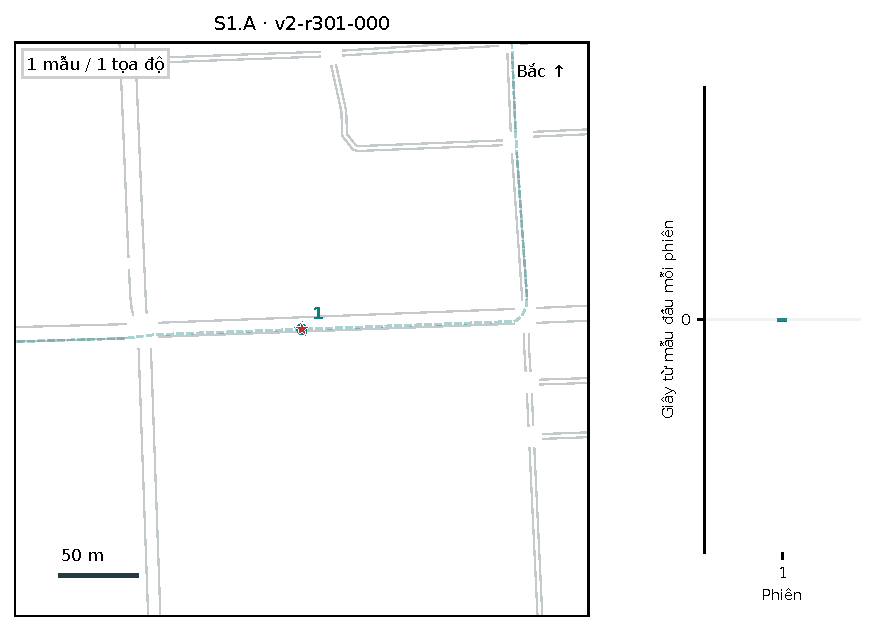
\includegraphics[width=\linewidth]{figures/case_S1_A.pdf}\end{minipage}\hfill\begin{minipage}[t]{0.42\linewidth}\vspace{0pt}\textbf{S1.A / 12 bản ghi.} Một bản tin tại cạnh có $\ge$2 hướng đi tiếp hợp lệ: kiểm tra khi mạng đường còn nhiều khả năng.\par\smallskip u301\_\allowbreak{}00: 1 mẫu\par\smallskip\textbf{Đọc sample.} Một lần lấy mẫu ở cạnh có 4 hướng đi tiếp. Sao đỏ trùng vị trí đầu vào; đối thủ phải chọn vị trí từ đầu ra đã bảo vệ, không được thấy sẵn sao này.\end{minipage}\par\vspace{3pt}
\noindent\begin{minipage}[t]{0.55\linewidth}\vspace{0pt}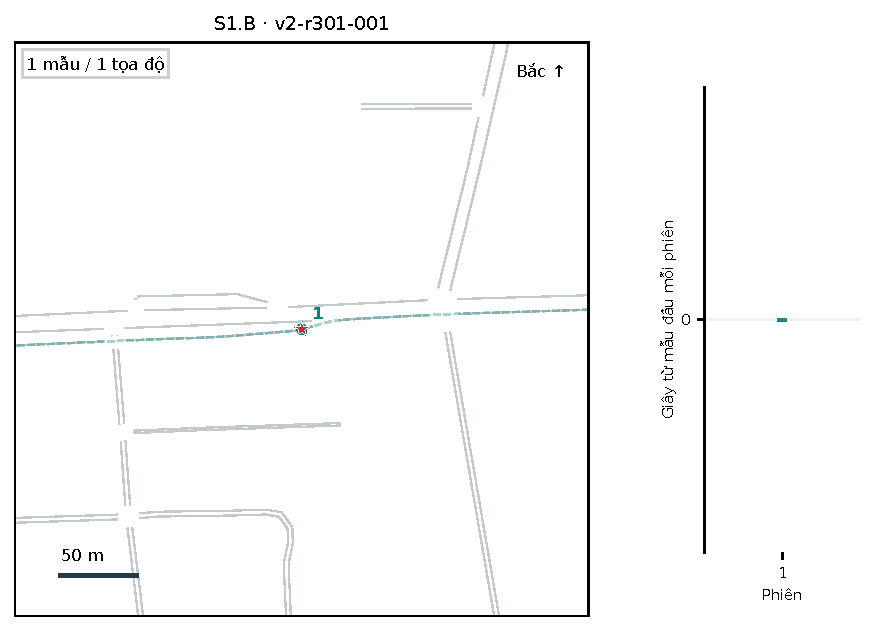
\includegraphics[width=\linewidth]{figures/case_S1_B.pdf}\end{minipage}\hfill\begin{minipage}[t]{0.42\linewidth}\vspace{0pt}\textbf{S1.B / 12 bản ghi.} Một bản tin tại cạnh chỉ có 1 hướng đi tiếp: bản đồ tự loại bớt khả năng.\par\smallskip u301\_\allowbreak{}00: 1 mẫu\par\smallskip\textbf{Đọc sample.} Vẫn chỉ một lần lấy mẫu, nhưng cạnh chỉ có một hướng đi tiếp. Bản đồ có thể loại bớt khả năng so với A; cần đo lợi thế này bằng đối thủ thực tế.\end{minipage}\par\vspace{3pt}
\noindent\begin{minipage}[t]{0.55\linewidth}\vspace{0pt}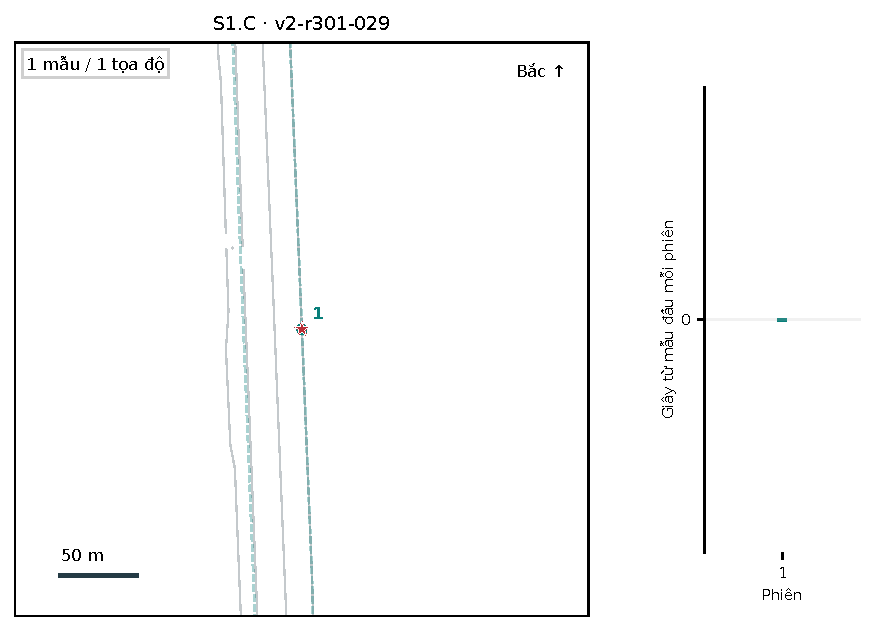
\includegraphics[width=\linewidth]{figures/case_S1_C.pdf}\end{minipage}\hfill\begin{minipage}[t]{0.42\linewidth}\vspace{0pt}\textbf{S1.C / 12 bản ghi.} Cách POI $\le$150 m; loại POI chiếm $\le$5\% danh mục công khai. Hiếm theo loại địa điểm, không phải theo tần suất ghé thăm.\par\smallskip u301\_\allowbreak{}13: 1 mẫu\par\smallskip\textbf{Đọc sample.} Điểm lấy mẫu cách POI pharmacy 12,03 m; loại này chiếm 3,11\% danh mục. Ngữ cảnh địa điểm hiếm là dấu hiệu bổ sung, không phải chuỗi di chuyển.\end{minipage}\par\vspace{3pt}

\clearpage
\subsection{S2 — suy ra nơi dừng qua nhiều lần gửi}
\textbf{Rủi ro chung:} Khác S1, đối thủ ghép nhiều lần gửi của cùng phiên để khoanh điểm dừng. Các chấm trùng vị trí không có nghĩa chỉ gửi một lần. Nhiễu độc lập có thể bị trung bình hóa; neo tái dùng cần được đánh giá riêng.

\noindent\begin{minipage}[t]{0.55\linewidth}\vspace{0pt}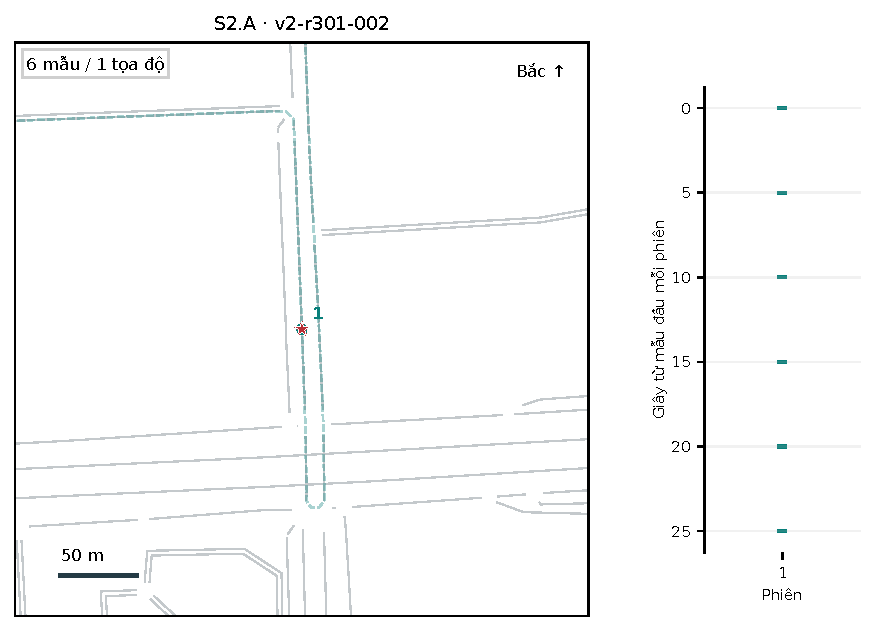
\includegraphics[width=\linewidth]{figures/case_S2_A.pdf}\end{minipage}\hfill\begin{minipage}[t]{0.42\linewidth}\vspace{0pt}\textbf{S2.A / 12 bản ghi.} Dừng có chủ đích $\ge$20 giây; lấy truy vấn mỗi 5 giây.\par\smallskip u301\_\allowbreak{}05: 6 mẫu\par\smallskip\textbf{Đọc sample.} 6 mẫu cùng một tọa độ, cách nhau 5 giây; đoạn dừng thật dài 29 giây. Sáu vạch thời gian bị chồng thành một chấm trên map.\end{minipage}\par\vspace{3pt}
\noindent\begin{minipage}[t]{0.55\linewidth}\vspace{0pt}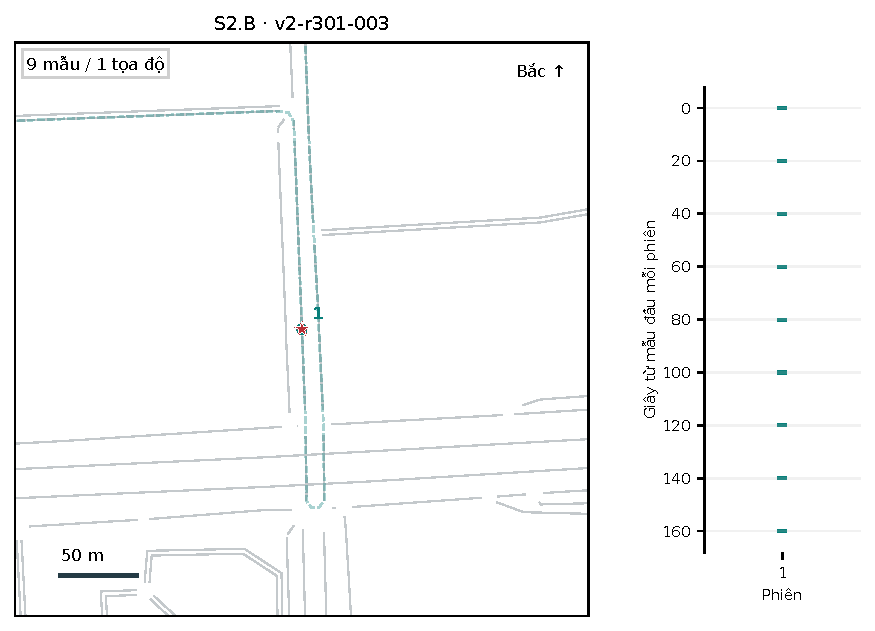
\includegraphics[width=\linewidth]{figures/case_S2_B.pdf}\end{minipage}\hfill\begin{minipage}[t]{0.42\linewidth}\vspace{0pt}\textbf{S2.B / 12 bản ghi.} Dừng $\ge$120 giây; lấy truy vấn mỗi 20 giây.\par\smallskip u301\_\allowbreak{}06: 9 mẫu\par\smallskip\textbf{Đọc sample.} 9 mẫu cùng một tọa độ, cách nhau 20 giây; đoạn dừng dài 179 giây. Đối thủ có cửa sổ dài hơn để kết hợp bằng chứng, không chỉ một bản tin.\end{minipage}\par\vspace{3pt}
\noindent\begin{minipage}[t]{0.55\linewidth}\vspace{0pt}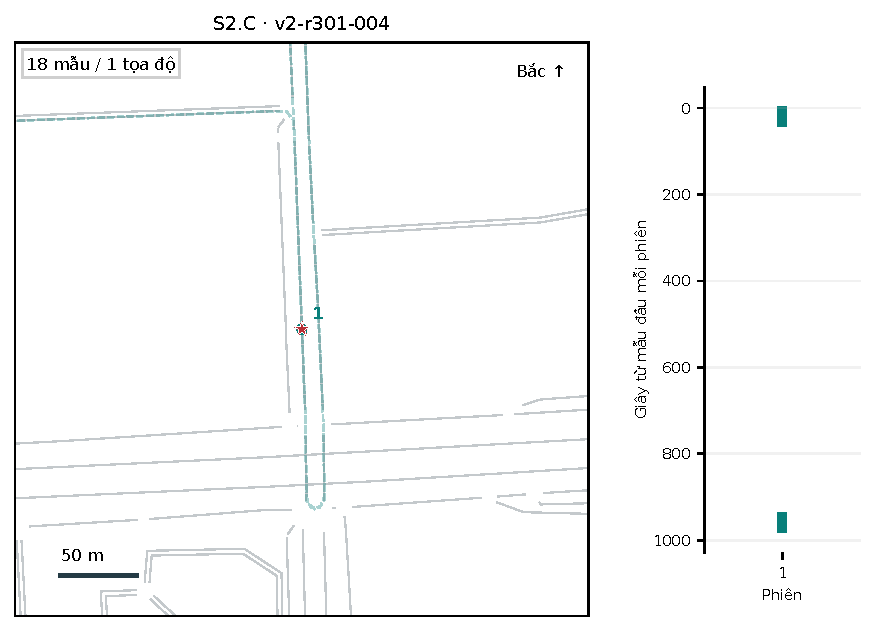
\includegraphics[width=\linewidth]{figures/case_S2_C.pdf}\end{minipage}\hfill\begin{minipage}[t]{0.42\linewidth}\vspace{0pt}\textbf{S2.C / 12 bản ghi.} Hai lần dừng trên cùng làn, mỗi lần $\ge$20 giây; ở giữa thực sự di chuyển.\par\smallskip u301\_\allowbreak{}07: 18 mẫu\par\smallskip\textbf{Đọc sample.} 18 mẫu chia hai đợt, mỗi đợt 9 mẫu. Hai lần dừng dài 44 giây tại cùng tọa độ; khoảng trống giữa hai cụm thời gian là lúc xe rời đi rồi quay lại.\end{minipage}\par\vspace{3pt}

\clearpage
\subsection{S3 — tái dựng đoạn đường đã đi}
\textbf{Rủi ro chung:} Đối thủ ghép các bản tin theo đường hợp lệ và thời gian di chuyển để tái dựng đoạn đã đi. Rủi ro nằm ở cả chuỗi: từng điểm mơ hồ vẫn có thể tạo ra một tuyến dễ đoán.

\noindent\begin{minipage}[t]{0.55\linewidth}\vspace{0pt}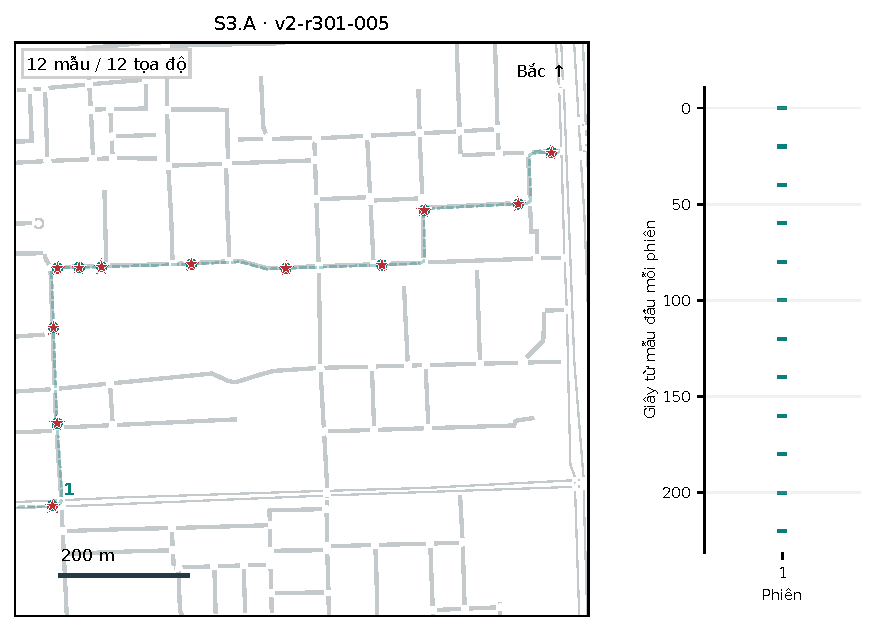
\includegraphics[width=\linewidth]{figures/case_S3_A.pdf}\end{minipage}\hfill\begin{minipage}[t]{0.42\linewidth}\vspace{0pt}\textbf{S3.A / 12 bản ghi.} Đoạn di chuyển $\ge$60 giây qua $\ge$3 cạnh; gửi mỗi 20 giây.\par\smallskip u301\_\allowbreak{}00: 12 mẫu\par\smallskip\textbf{Đọc sample.} 12 mẫu của u301\_\allowbreak{}00 cách nhau 20 giây. Chuỗi điểm cung cấp nhiều ràng buộc để nối tuyến; nét đứt là đường thật chỉ dùng chấm.\end{minipage}\par\vspace{3pt}
\noindent\begin{minipage}[t]{0.55\linewidth}\vspace{0pt}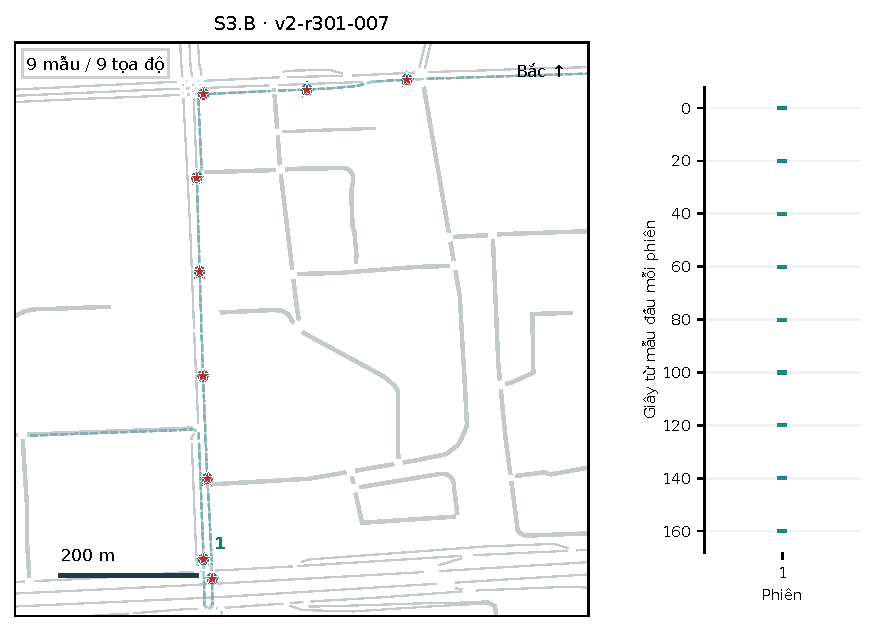
\includegraphics[width=\linewidth]{figures/case_S3_B.pdf}\end{minipage}\hfill\begin{minipage}[t]{0.42\linewidth}\vspace{0pt}\textbf{S3.B / 11 bản ghi.} Ít nhất một nửa số cạnh được lấy mẫu chỉ có một hướng đi tiếp: hành lang ít lựa chọn.\par\smallskip u301\_\allowbreak{}00: 9 mẫu\par\smallskip\textbf{Đọc sample.} 9 mẫu; 55,6\% cạnh được lấy mẫu chỉ có một hướng đi tiếp. Đường ít nhánh có thể khiến chuỗi dễ suy hơn dù từng vị trí được làm mờ.\end{minipage}\par\vspace{3pt}
\noindent\begin{minipage}[t]{0.55\linewidth}\vspace{0pt}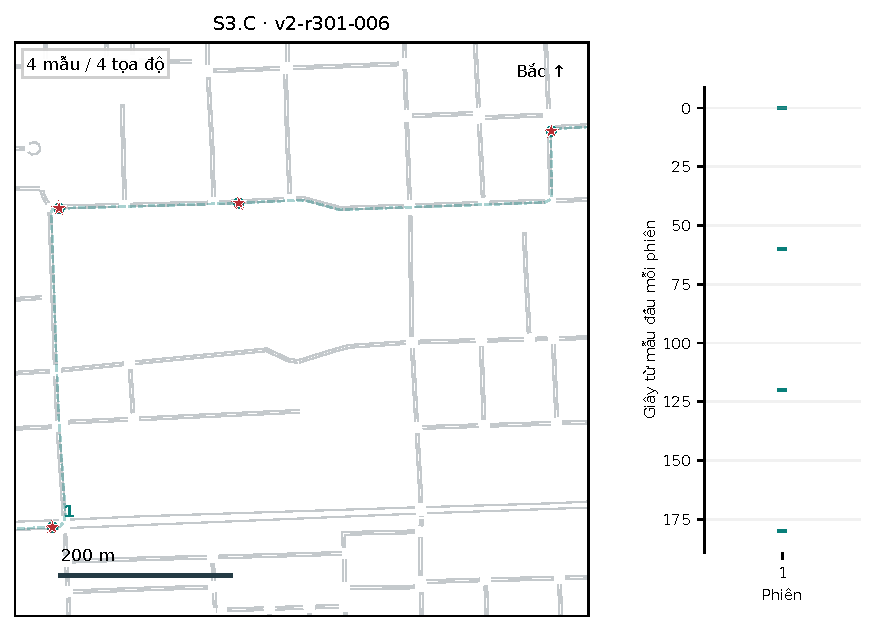
\includegraphics[width=\linewidth]{figures/case_S3_C.pdf}\end{minipage}\hfill\begin{minipage}[t]{0.42\linewidth}\vspace{0pt}\textbf{S3.C / 12 bản ghi.} Lấy mẫu đoạn di chuyển thưa hơn, mỗi 60 giây.\par\smallskip u301\_\allowbreak{}00: 4 mẫu\par\smallskip\textbf{Đọc sample.} 4 mẫu của cùng đoạn trong A, cách nhau 60 giây. Khoảng trống lớn hơn nhưng đối thủ vẫn có thể dùng mạng đường để nối các khả năng.\end{minipage}\par\vspace{3pt}

\clearpage
\subsection{S9 — suy ra điểm xuất phát bị che}
\textbf{Rủi ro chung:} Từ phần sau được công bố, đối thủ suy ngược nơi xuất phát nhờ đường vào/ra và phiên lặp. Hai sao bị che ở B là hai khả năng phải phân biệt; không phải bản đồ đã chứng minh đoán đúng.

\noindent\begin{minipage}[t]{0.55\linewidth}\vspace{0pt}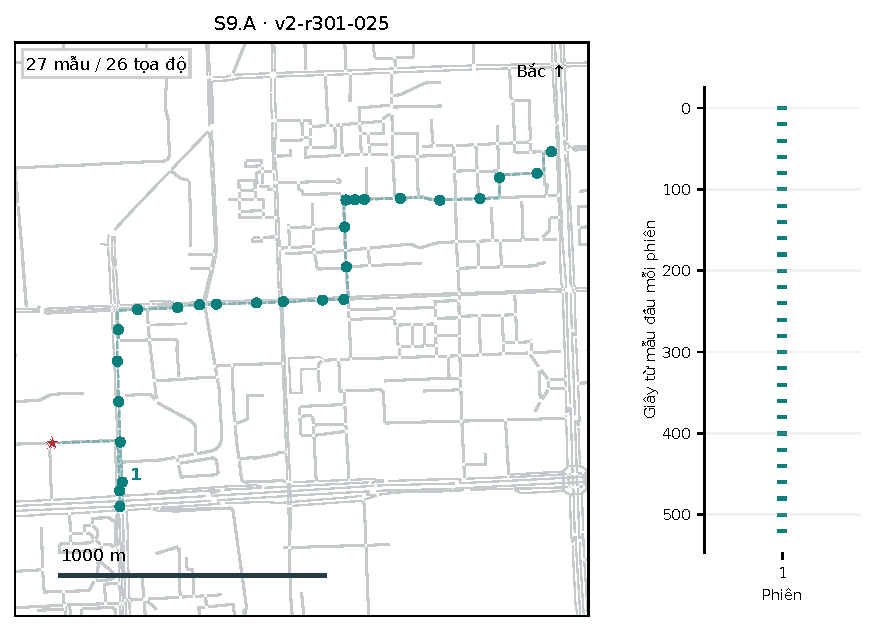
\includegraphics[width=\linewidth]{figures/case_S9_A.pdf}\end{minipage}\hfill\begin{minipage}[t]{0.42\linewidth}\vspace{0pt}\textbf{S9.A / 12 bản ghi.} Cạnh xuất phát chỉ một lối ra. Che 60 giây đầu, lấy phần còn lại mỗi 20 giây.\par\smallskip u301\_\allowbreak{}00: 27 mẫu\par\smallskip\textbf{Đọc sample.} Sao là FCD[0]; cửa sổ bắt đầu ở FCD[60] sau khi che 60 giây. Chỉ một lối ra có thể giúp suy ngược nguồn xuất phát từ phần còn công bố.\end{minipage}\par\vspace{3pt}
\noindent\begin{minipage}[t]{0.55\linewidth}\vspace{0pt}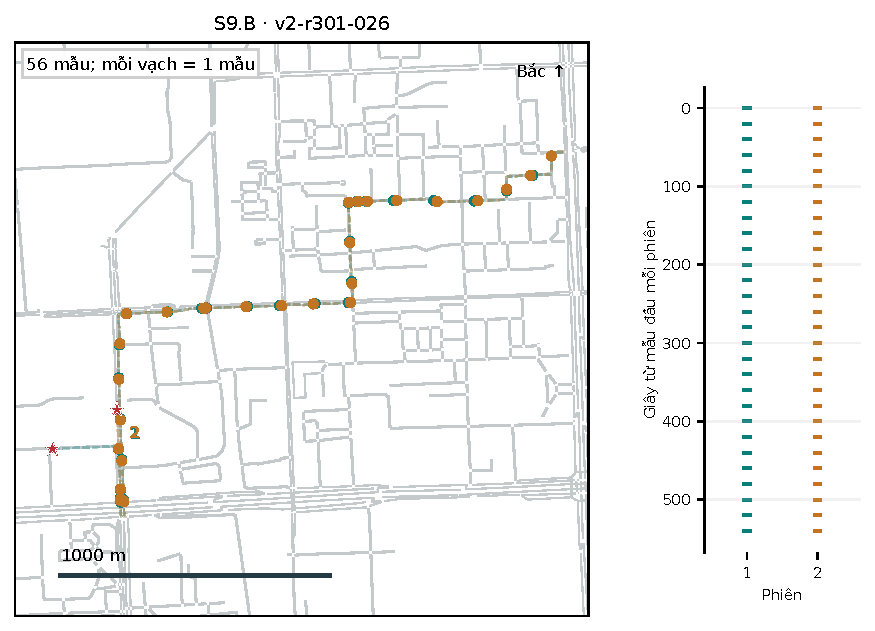
\includegraphics[width=\linewidth]{figures/case_S9_B.pdf}\end{minipage}\hfill\begin{minipage}[t]{0.42\linewidth}\vspace{0pt}\textbf{S9.B / 11 bản ghi.} Hai chuyến khác điểm đầu nhưng nhập một đoạn chung; chỉ cấp từ chỗ nhập tuyến.\par\smallskip u301\_\allowbreak{}00: 28 mẫu; u301\_\allowbreak{}04: 28 mẫu\par\smallskip\textbf{Đọc sample.} Hai điểm đầu cách 281,76 m rồi nhập tuyến. Chỉ cấp dữ liệu sau nhập; hai sao là hai đáp án bị giấu mà đối thủ phải phân biệt.\end{minipage}\par\vspace{3pt}
\noindent\begin{minipage}[t]{0.55\linewidth}\vspace{0pt}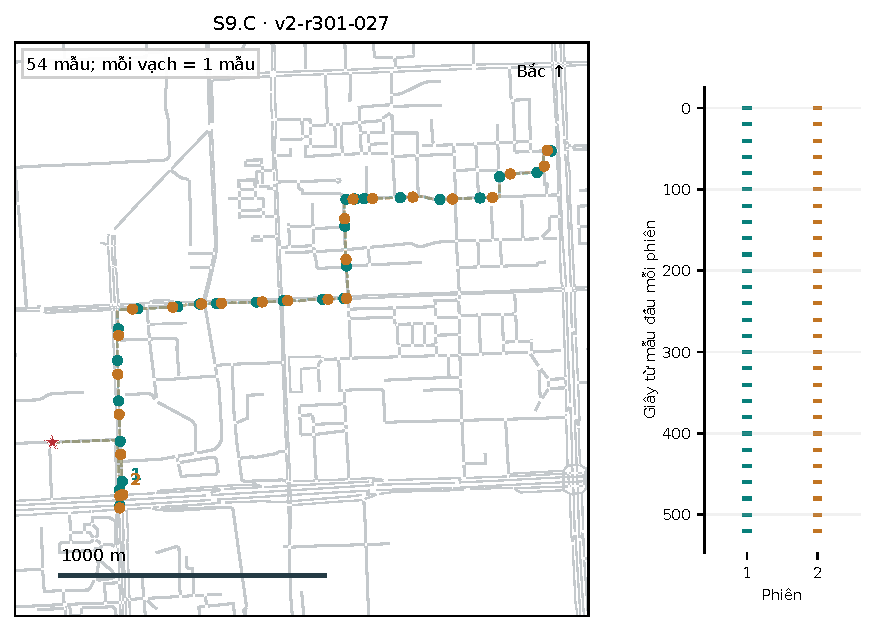
\includegraphics[width=\linewidth]{figures/case_S9_C.pdf}\end{minipage}\hfill\begin{minipage}[t]{0.42\linewidth}\vspace{0pt}\textbf{S9.C / 12 bản ghi.} Nhiều chuyến có cùng điểm xuất phát dự kiến; che 60 giây đầu từng chuyến.\par\smallskip u301\_\allowbreak{}00: 27 mẫu; u301\_\allowbreak{}09: 27 mẫu\par\smallskip\textbf{Đọc sample.} u301\_\allowbreak{}00/u301\_\allowbreak{}09 lặp cùng điểm đầu dự kiến; mỗi phiên che 60 giây đầu. Nhiều cửa sổ có thể bổ sung bằng chứng về cùng nguồn xuất phát.\end{minipage}\par\vspace{3pt}

\clearpage
\subsection{S10 — suy ra điểm kết thúc bị che}
\textbf{Rủi ro chung:} Đối thủ suy nơi đã kết thúc từ phần còn được công bố. A kiểm tra một chuyến với ràng buộc đường vào; C kiểm tra các phiên lặp cùng đích. Cả hai che 60 giây cuối.

\textbf{Hai ca cần giải quyết:} A suy endpoint từ phần cuối còn nhìn thấy và mạng đường; C còn kết hợp các chuyến lặp cùng đích. Giữ mã A/C để truy nguyên dữ liệu. Bài toán chung tiền tố nhưng khác đích thuộc S6.A.

\noindent\begin{minipage}[t]{0.63\linewidth}\vspace{0pt}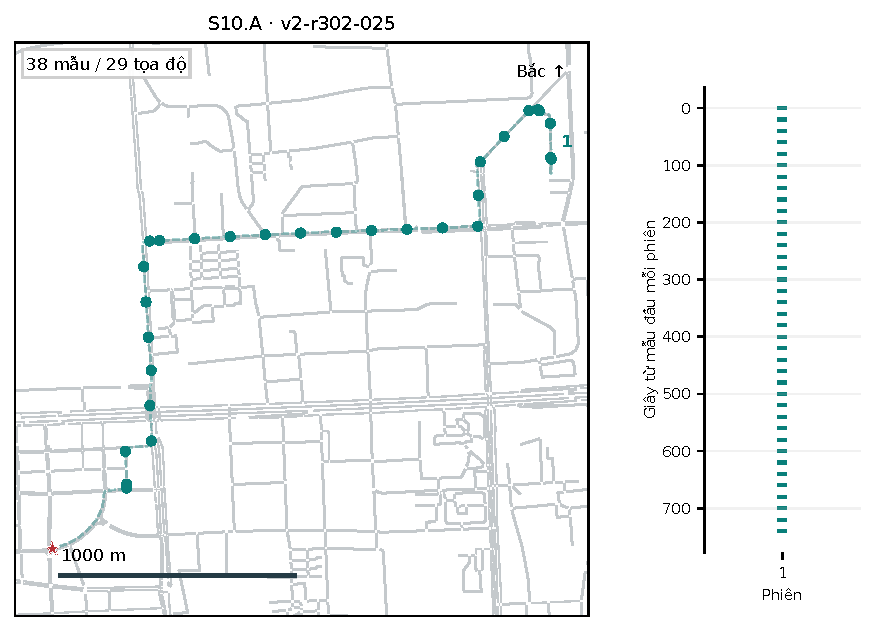
\includegraphics[width=\linewidth]{figures/case_S10_A.pdf}\end{minipage}\hfill\begin{minipage}[t]{0.34\linewidth}\vspace{0pt}\textbf{S10.A / 11 bản ghi.} Cạnh kết thúc chỉ một lối vào. Che 60 giây cuối của chuyến đã hoàn tất.\par\smallskip u302\_\allowbreak{}08: 38 mẫu\par\smallskip\textbf{Đọc sample.} Sao là FCD cuối [817] của u302\_\allowbreak{}08; che 60 giây cuối. Đường chỉ một lối vào có thể giúp suy đoạn kết thúc từ phần trước còn thấy.\end{minipage}\par\vspace{3pt}
\noindent\begin{minipage}[t]{0.63\linewidth}\vspace{0pt}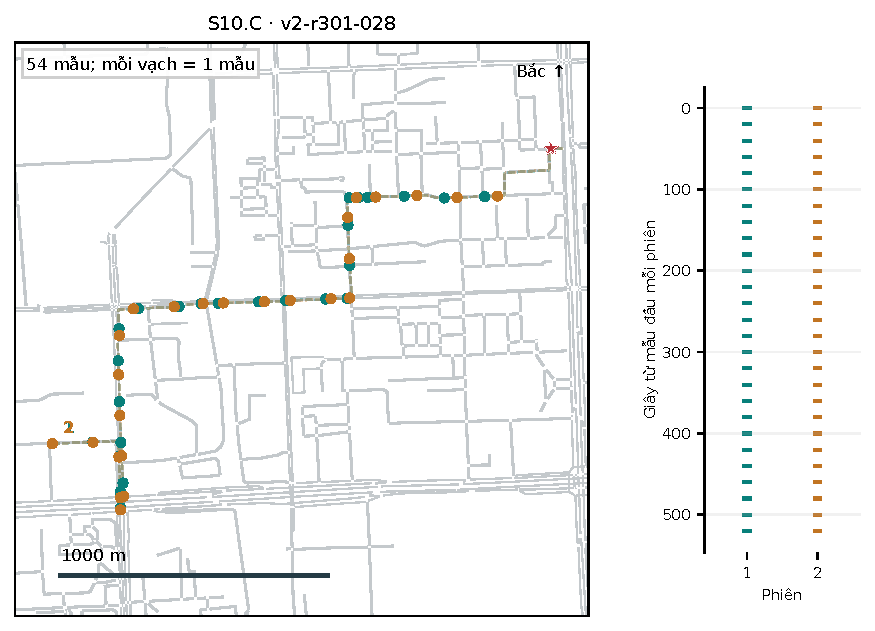
\includegraphics[width=\linewidth]{figures/case_S10_C.pdf}\end{minipage}\hfill\begin{minipage}[t]{0.34\linewidth}\vspace{0pt}\textbf{S10.C / 12 bản ghi.} Nhiều chuyến cùng điểm kết thúc dự kiến; che 60 giây cuối từng chuyến.\par\smallskip u301\_\allowbreak{}00: 27 mẫu; u301\_\allowbreak{}09: 27 mẫu\par\smallskip\textbf{Đọc sample.} u301\_\allowbreak{}00/u301\_\allowbreak{}09 lặp cùng đích dự kiến và cùng che 60 giây cuối. Đối thủ có thể kết hợp nhiều phiên để khoanh đích, chưa đủ gọi đó là nơi làm việc.\end{minipage}\par\vspace{3pt}

\clearpage
\subsection{S5 — dự đoán cạnh đường kế tiếp}
\textbf{Rủi ro chung:} Đối thủ dùng tiền tố và ngã rẽ để đoán cạnh kế tiếp chưa được công bố. Không cần biết tên xe. Phải so với mức đoán chỉ từ bản đồ, nhất là ca một lối đi.

\noindent\begin{minipage}[t]{0.55\linewidth}\vspace{0pt}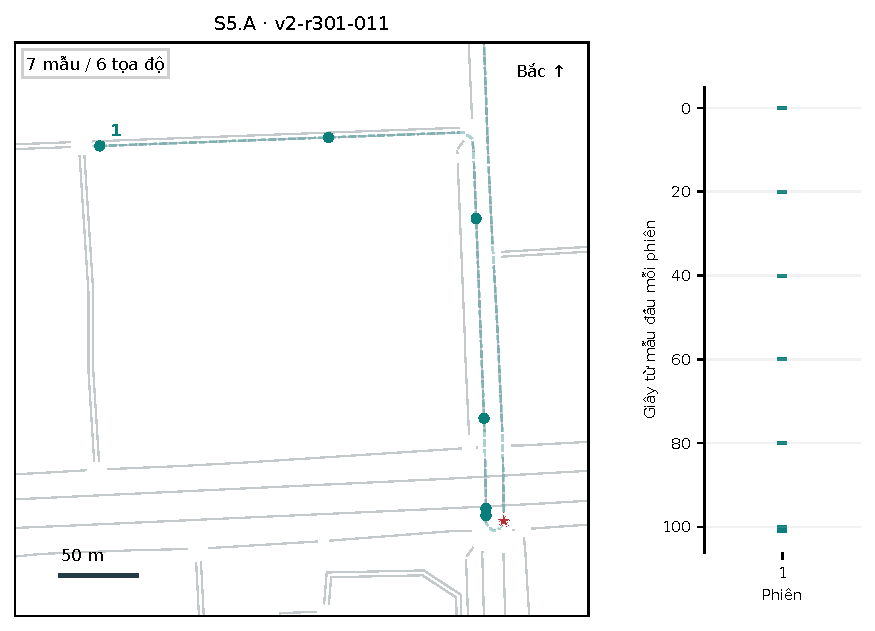
\includegraphics[width=\linewidth]{figures/case_S5_A.pdf}\end{minipage}\hfill\begin{minipage}[t]{0.42\linewidth}\vspace{0pt}\textbf{S5.A / 12 bản ghi.} Chỉ tiền tố trước một lượt rẽ có $\ge$2 lựa chọn; nhãn là cạnh kế tiếp thực sự đi vào.\par\smallskip u301\_\allowbreak{}00: 7 mẫu\par\smallskip\textbf{Đọc sample.} 7 mẫu tiền tố; nhãn tương lai ở FCD[106], cạnh 1055449630. Có nhiều lựa chọn tại lượt rẽ, nên phải dự đoán cạnh thật sự được chọn.\end{minipage}\par\vspace{3pt}
\noindent\begin{minipage}[t]{0.55\linewidth}\vspace{0pt}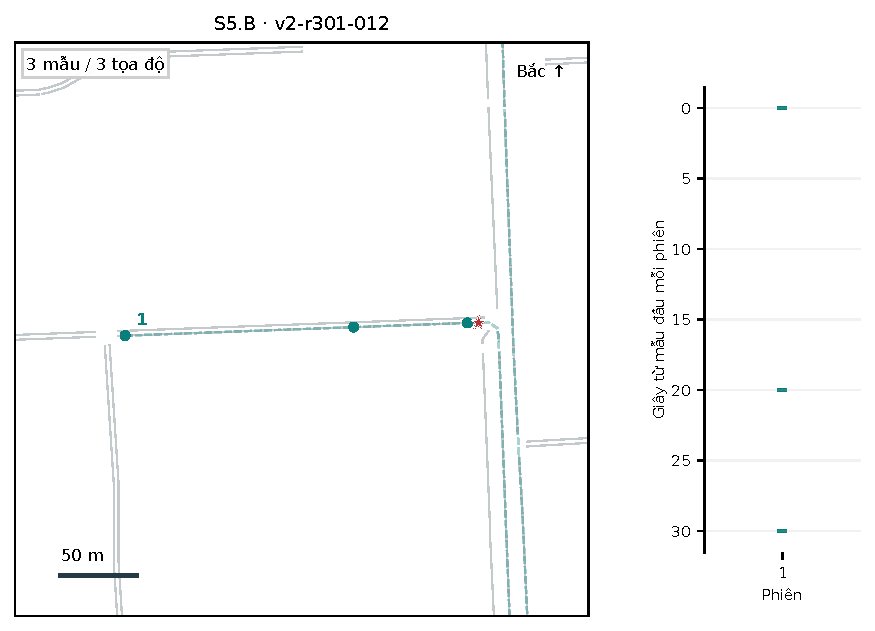
\includegraphics[width=\linewidth]{figures/case_S5_B.pdf}\end{minipage}\hfill\begin{minipage}[t]{0.42\linewidth}\vspace{0pt}\textbf{S5.B / 12 bản ghi.} Lượt chuyển chỉ có 1 lựa chọn; kiểm tra mức suy luận vốn đã có từ bản đồ.\par\smallskip u301\_\allowbreak{}00: 3 mẫu\par\smallskip\textbf{Đọc sample.} 3 mẫu tiền tố; nhãn ở FCD[31], cạnh 177353867\#16. Lượt chuyển chỉ có một lựa chọn: phải so với mức đoán nền từ bản đồ.\end{minipage}\par\vspace{3pt}
\noindent\begin{minipage}[t]{0.55\linewidth}\vspace{0pt}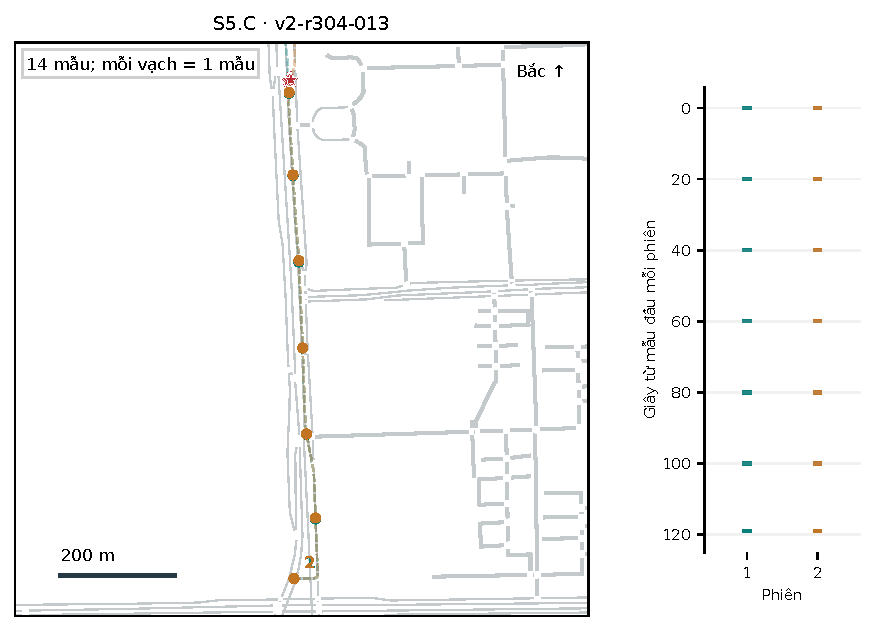
\includegraphics[width=\linewidth]{figures/case_S5_C.pdf}\end{minipage}\hfill\begin{minipage}[t]{0.42\linewidth}\vspace{0pt}\textbf{S5.C / 4 bản ghi.} Hai chuyến chung tiền tố tuyến kế hoạch nhưng đi vào hai cạnh khác nhau. Tốc độ và thời điểm không bắt buộc giống hệt.\par\smallskip u304\_\allowbreak{}00: 7 mẫu; u304\_\allowbreak{}02: 7 mẫu\par\smallskip\textbf{Đọc sample.} Mỗi phiên có 7 mẫu tiền tố tới FCD[119], rồi vào hai cạnh khác nhau tại FCD[122]. Hai sao gần nhau vẫn có thể thuộc hai nhãn cạnh khác nhau.\end{minipage}\par\vspace{3pt}

\clearpage
\subsection{S6 — dự đoán đích chưa tới}
\textbf{Rủi ro chung:} Đối thủ dự đoán đích từ tiền tố và lịch sử được phép. Năm lần tới một đích không đảm bảo chuyến mới cũng vậy; cần so với tần suất nền. Rủi ro là biết nơi sắp đến trước khi chuyến kết thúc.

\noindent\begin{minipage}[t]{0.55\linewidth}\vspace{0pt}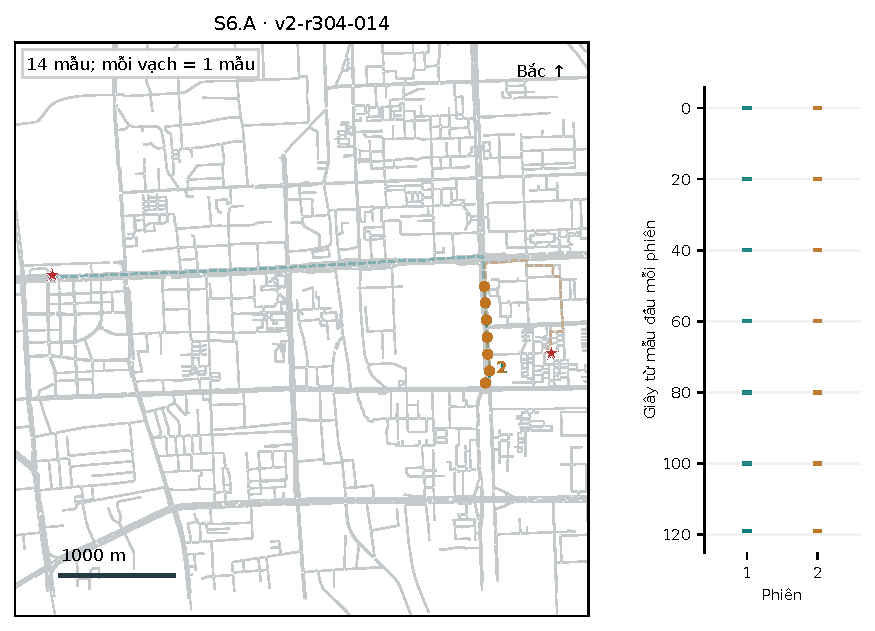
\includegraphics[width=\linewidth]{figures/case_S6_A.pdf}\end{minipage}\hfill\begin{minipage}[t]{0.42\linewidth}\vspace{0pt}\textbf{S6.A / 4 bản ghi.} Hai chuyến chung tiền tố nhưng có đích khác nhau; phần sau không được cấp.\par\smallskip u304\_\allowbreak{}00: 7 mẫu; u304\_\allowbreak{}02: 7 mẫu\par\smallskip\textbf{Đọc sample.} Hai tiền tố của u304\_\allowbreak{}00/u304\_\allowbreak{}02 dẫn tới hai đích cách 4,47 km. Hai sao là đích tương lai giữ kín; tiền tố chưa quyết định một đích duy nhất.\end{minipage}\par\vspace{3pt}
\noindent\begin{minipage}[t]{0.55\linewidth}\vspace{0pt}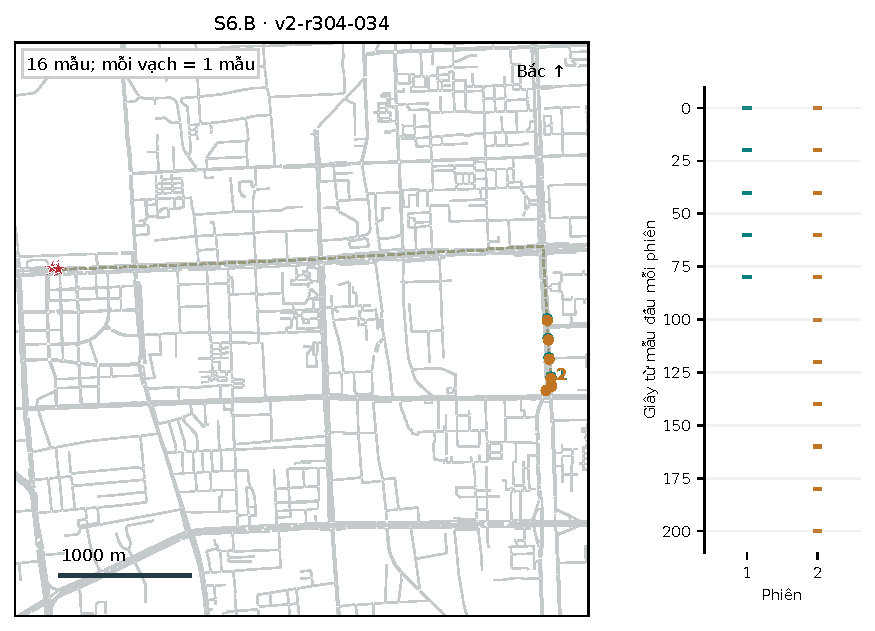
\includegraphics[width=\linewidth]{figures/case_S6_B.pdf}\end{minipage}\hfill\begin{minipage}[t]{0.42\linewidth}\vspace{0pt}\textbf{S6.B / 5 bản ghi.} Hai đích cách nhau $\le$500 m: phân biệt đúng đích có thể khó dù sai số tọa độ nhỏ.\par\smallskip u304\_\allowbreak{}00: 5 mẫu; u304\_\allowbreak{}12: 11 mẫu\par\smallskip\textbf{Đọc sample.} u304\_\allowbreak{}00/u304\_\allowbreak{}12 có hai đích chỉ cách 46,21 m. Dự đoán gần về tọa độ có thể vẫn chọn sai đích: cần chấm cả hai khía cạnh.\end{minipage}\par\vspace{3pt}
\noindent\begin{minipage}[t]{0.55\linewidth}\vspace{0pt}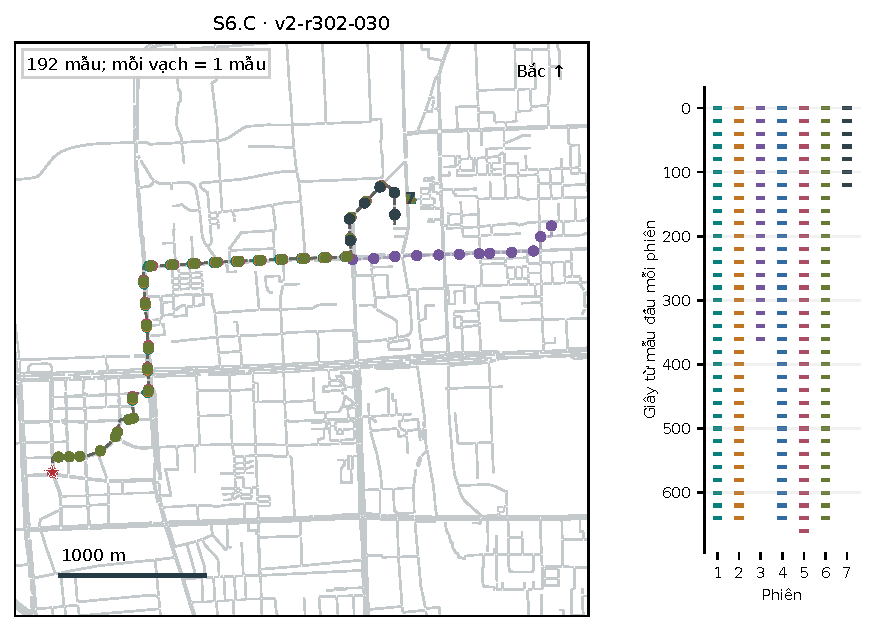
\includegraphics[width=\linewidth]{figures/case_S6_C.pdf}\end{minipage}\hfill\begin{minipage}[t]{0.42\linewidth}\vspace{0pt}\textbf{S6.C / 10 bản ghi.} Sáu chuyến lịch sử: 5 tới đích thường, 1 tới đích hiếm; chỉ tiền tố của chuyến hiện tại. Lịch sử phải được bảo vệ trước khi cấp.\par\smallskip 6 phiên lịch sử + phiên hiện tại: 7 mẫu tiền tố.\par\smallskip\textbf{Đọc sample.} Sáu chuyến lịch sử: 5 đích thường, 1 đích hiếm. Phiên thứ bảy chỉ cấp 7 mẫu tiền tố; phải phân biệt suy từ transcript với đoán theo tần suất lịch sử.\end{minipage}\par\vspace{3pt}

\clearpage
\subsection{S8 — định vị khi có dữ liệu người đi cùng}
\textbf{Rủi ro chung:} Vị trí xe phụ trợ có thể thu hẹp vị trí xe mục tiêu khi chúng đi gần nhau. So độ định vị có/không có phụ trợ. Ca C kiểm tra bẫy ‘ở gần tức là đồng hành’; hình chưa chứng minh tấn công thành công.

\noindent\begin{minipage}[t]{0.55\linewidth}\vspace{0pt}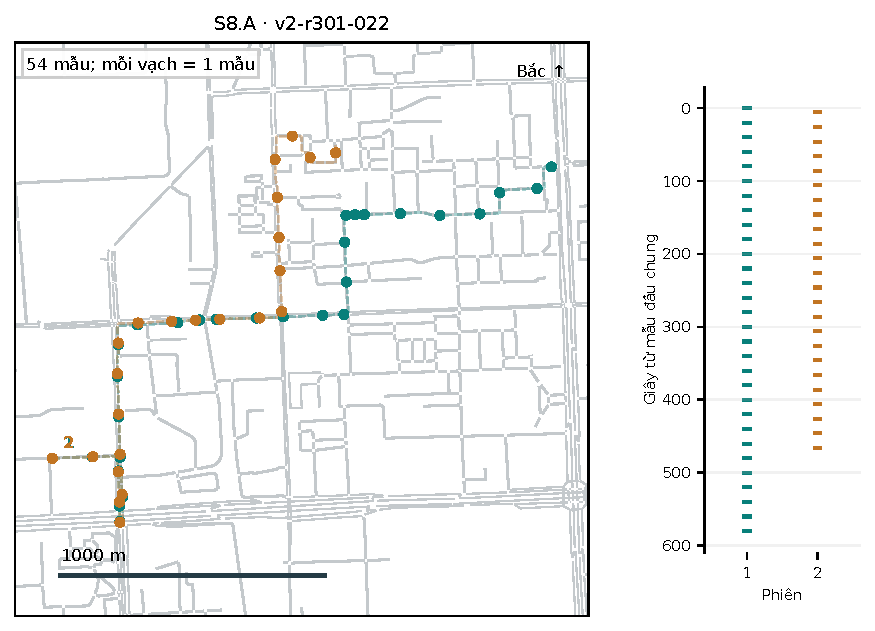
\includegraphics[width=\linewidth]{figures/case_S8_A.pdf}\end{minipage}\hfill\begin{minipage}[t]{0.42\linewidth}\vspace{0pt}\textbf{S8.A / 12 bản ghi.} Đi cùng một phần rồi tách; ở gần $\le$100 m trong $\ge$10 giây liên tục.\par\smallskip u301\_\allowbreak{}00: 30 mẫu; u301\_\allowbreak{}02: 24 mẫu\par\smallskip\textbf{Đọc sample.} Hai xe có nhãn đồng hành, gần nhau ở 325/466 thời điểm đồng bộ. Dữ liệu xe phụ trợ có thể giúp định vị ở đoạn đi chung; sau tách tuyến lợi thế có thể đổi.\end{minipage}\par\vspace{3pt}
\noindent\begin{minipage}[t]{0.55\linewidth}\vspace{0pt}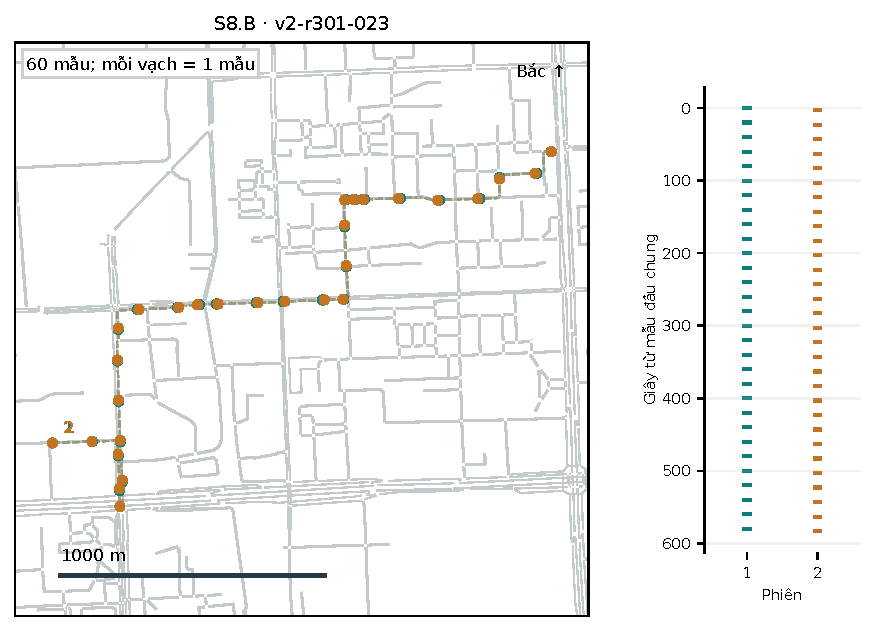
\includegraphics[width=\linewidth]{figures/case_S8_B.pdf}\end{minipage}\hfill\begin{minipage}[t]{0.42\linewidth}\vspace{0pt}\textbf{S8.B / 9 bản ghi.} Chung tuyến; $\ge$80\% thời điểm đồng xuất hiện cách $\le$100 m, có $\ge$10 giây liên tục ở gần.\par\smallskip u301\_\allowbreak{}00: 30 mẫu; u301\_\allowbreak{}01: 30 mẫu\par\smallskip\textbf{Đọc sample.} Hai xe có nhãn đồng hành và gần nhau ở 590/590 thời điểm đồng bộ. Đây là mẫu để kiểm tra nguy cơ phụ trợ kéo dài gần suốt cửa sổ.\end{minipage}\par\vspace{3pt}
\noindent\begin{minipage}[t]{0.55\linewidth}\vspace{0pt}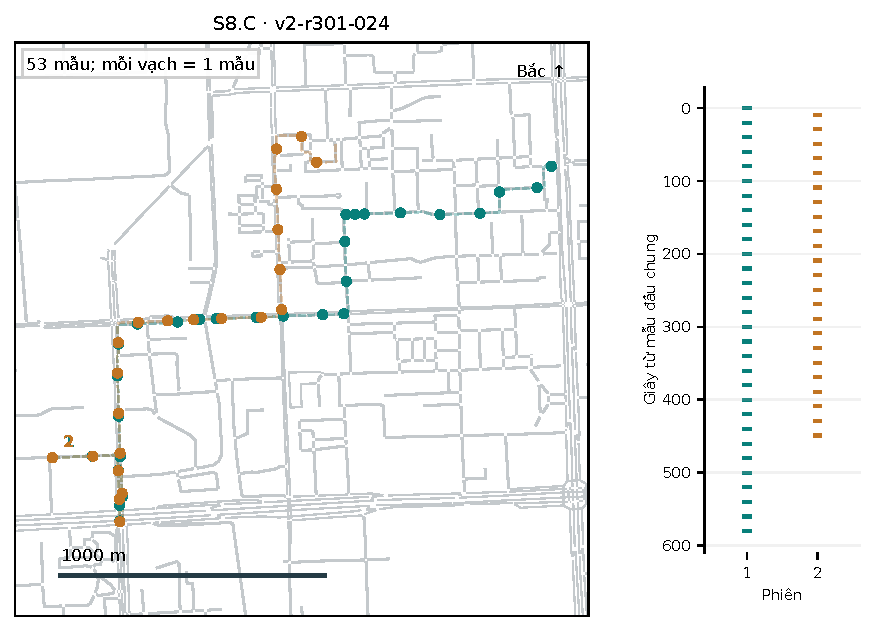
\includegraphics[width=\linewidth]{figures/case_S8_C.pdf}\end{minipage}\hfill\begin{minipage}[t]{0.42\linewidth}\vspace{0pt}\textbf{S8.C / 12 bản ghi.} Không gán quan hệ đồng hành nhưng tình cờ ở gần; đối chứng âm.\par\smallskip u301\_\allowbreak{}00: 30 mẫu; u301\_\allowbreak{}03: 23 mẫu\par\smallskip\textbf{Đọc sample.} Không gán đồng hành nhưng vẫn gần nhau ở 309/460 thời điểm. Mẫu âm kiểm tra giả định ‘ở gần tức đi cùng’; mục tiêu vẫn là định vị xe khi có/không có phụ trợ.\end{minipage}\par\vspace{3pt}

\clearpage
\subsection{S4 — liên kết danh tính giữa các phiên}
\textbf{Rủi ro chung:} Đối thủ tìm dấu hiệu tuyến/lịch lặp để nối hai phiên dù đổi mã hoặc thiết bị. Liên kết làm lộ lịch sử cùng chủ thể; biết tên thật còn cần bằng chứng phụ. Màu session không phải nhãn người.

\noindent\begin{minipage}[t]{0.55\linewidth}\vspace{0pt}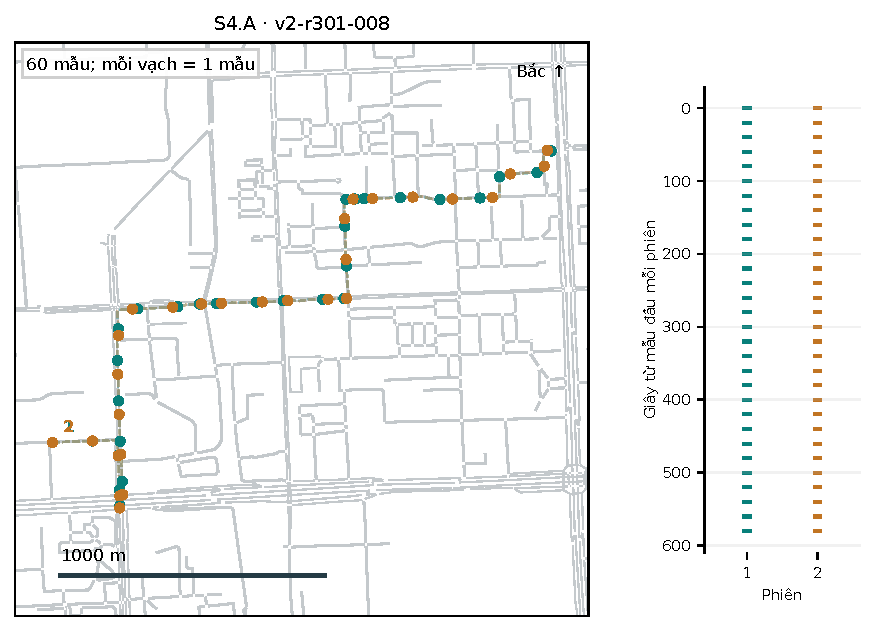
\includegraphics[width=\linewidth]{figures/case_S4_A.pdf}\end{minipage}\hfill\begin{minipage}[t]{0.42\linewidth}\vspace{0pt}\textbf{S4.A / 12 bản ghi.} Hai phiên không chồng lấn, cùng người và cùng thiết bị.\par\smallskip u301\_\allowbreak{}00: 30 mẫu; u301\_\allowbreak{}09: 30 mẫu\par\smallskip\textbf{Đọc sample.} u301\_\allowbreak{}00 và u301\_\allowbreak{}09 cùng người, cùng thiết bị. Hai màu là hai phiên, không phải hai người; mẫu kiểm tra khả năng nối lại chúng.\end{minipage}\par\vspace{3pt}
\noindent\begin{minipage}[t]{0.55\linewidth}\vspace{0pt}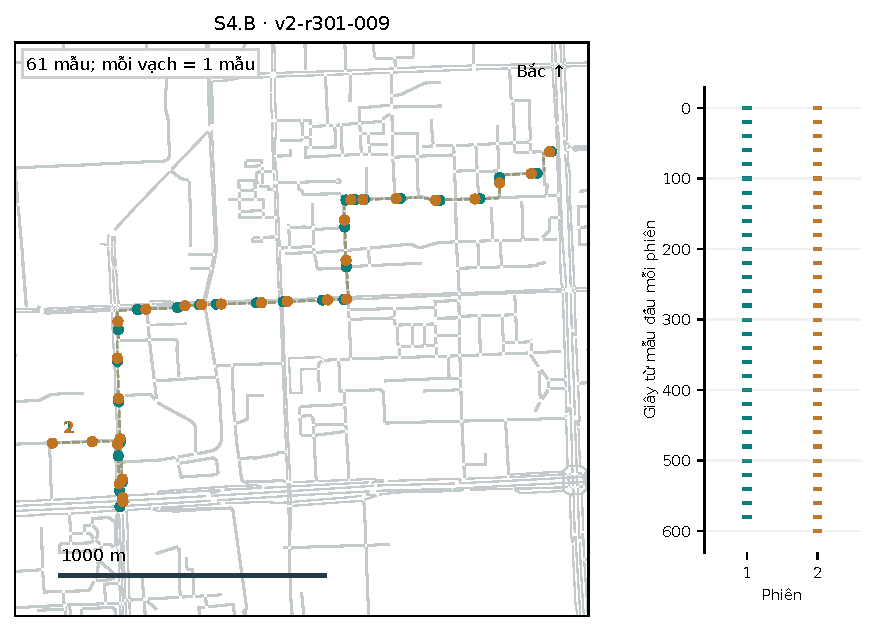
\includegraphics[width=\linewidth]{figures/case_S4_B.pdf}\end{minipage}\hfill\begin{minipage}[t]{0.42\linewidth}\vspace{0pt}\textbf{S4.B / 12 bản ghi.} Cùng người nhưng đổi thiết bị: liên kết người đúng, liên kết thiết bị sai.\par\smallskip u301\_\allowbreak{}00: 30 mẫu; u301\_\allowbreak{}10: 31 mẫu\par\smallskip\textbf{Đọc sample.} u301\_\allowbreak{}00 và u301\_\allowbreak{}10 cùng người nhưng khác thiết bị. Nếu đối thủ vẫn nối được từ tuyến/lịch, đổi thiết bị chưa đủ ngăn theo dõi người.\end{minipage}\par\vspace{3pt}
\noindent\begin{minipage}[t]{0.55\linewidth}\vspace{0pt}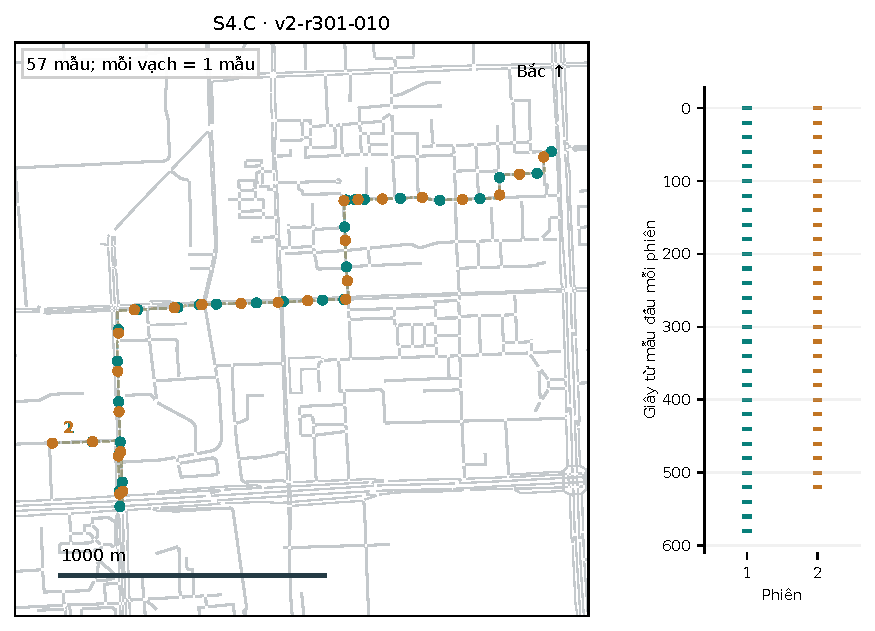
\includegraphics[width=\linewidth]{figures/case_S4_C.pdf}\end{minipage}\hfill\begin{minipage}[t]{0.42\linewidth}\vspace{0pt}\textbf{S4.C / 12 bản ghi.} Khác người nhưng dùng chung thiết bị: liên kết người sai, liên kết thiết bị đúng.\par\smallskip u301\_\allowbreak{}00: 30 mẫu; u301\_\allowbreak{}11: 27 mẫu\par\smallskip\textbf{Đọc sample.} u301\_\allowbreak{}00 và u301\_\allowbreak{}11 khác người nhưng cùng thiết bị. Gộp hai phiên theo thiết bị sẽ đúng ở mức thiết bị nhưng sai ở mức người.\end{minipage}\par\vspace{3pt}

\clearpage
\subsection{S7 — suy ra nội dung hoặc ý định truy vấn}
\textbf{Rủi ro chung:} Rủi ro nằm ở nội dung: pharmacy $\to$ clinic $\to$ hospital có thể gợi ý mục đích khám bệnh dù vị trí mờ. Đây là suy ý định, không chẩn đoán bệnh; nhãn hiện tại được gán tổng hợp.

\noindent\begin{minipage}[t]{0.55\linewidth}\vspace{0pt}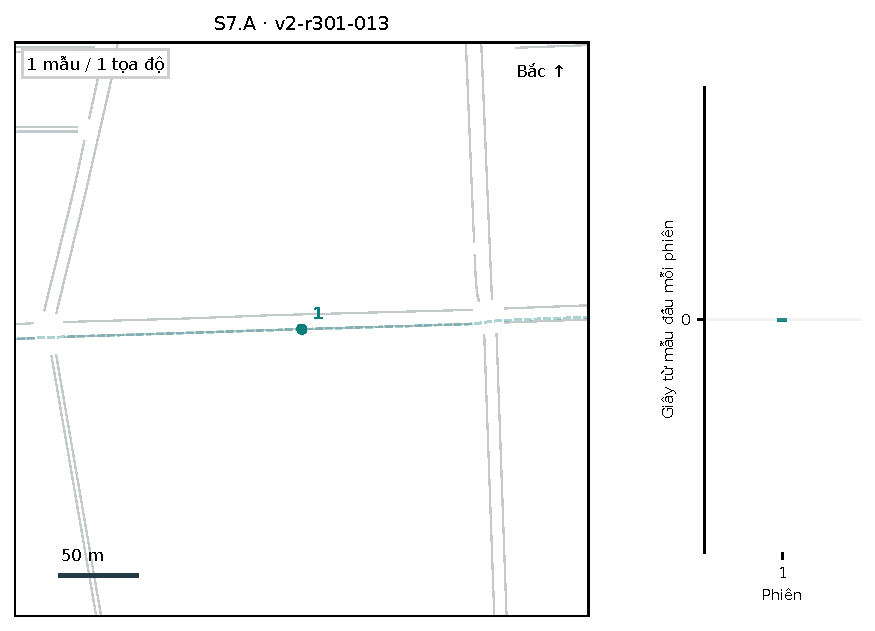
\includegraphics[width=\linewidth]{figures/case_S7_A.pdf}\end{minipage}\hfill\begin{minipage}[t]{0.42\linewidth}\vspace{0pt}\textbf{S7.A / 36 bản ghi.} Gửi nguyên văn; nhãn tổng hợp gồm khám bệnh, mua sắm, đi đường dài.\par\smallskip u301\_\allowbreak{}00: 1 mẫu\par\smallskip\textbf{Đọc sample.} Một lần query clinic, nhãn ý định tổng hợp medical\_\allowbreak{}visit. Ngay cả khi giấu vị trí, nội dung nguyên văn vẫn có thể gợi ý nhu cầu.\end{minipage}\par\vspace{3pt}
\noindent\begin{minipage}[t]{0.55\linewidth}\vspace{0pt}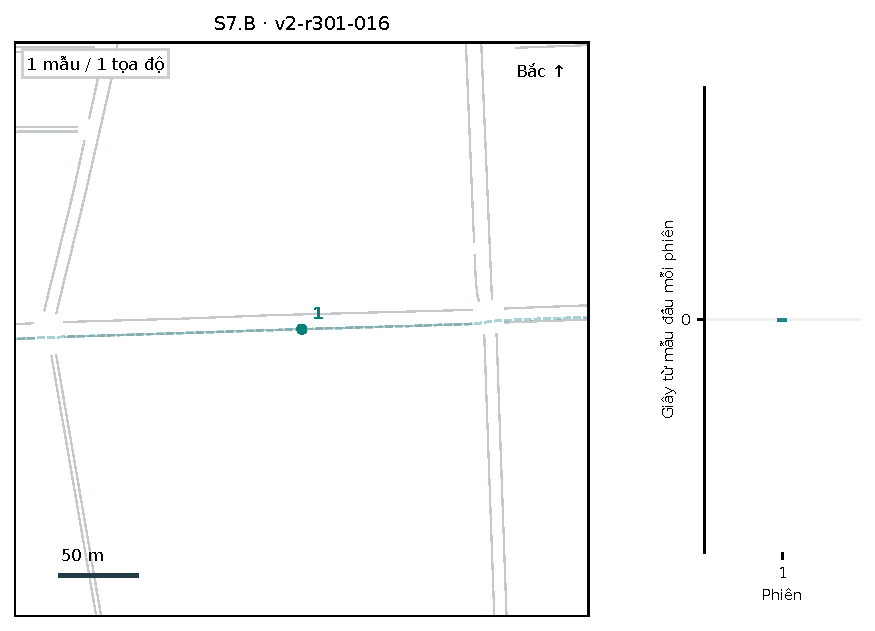
\includegraphics[width=\linewidth]{figures/case_S7_B.pdf}\end{minipage}\hfill\begin{minipage}[t]{0.42\linewidth}\vspace{0pt}\textbf{S7.B / 36 bản ghi.} Trộn truy vấn thật trong bó cố định 6 loại; chính sách tham chiếu, chưa phải đầu ra BR-Dummy.\par\smallskip u301\_\allowbreak{}00: 1 mẫu\par\smallskip\textbf{Đọc sample.} Cùng query thật clinic nhưng bó công bố gồm 6 loại. Đối thủ không nhận cờ query thật; map giống A vì khác biệt nằm ở nội dung gửi.\end{minipage}\par\vspace{3pt}
\noindent\begin{minipage}[t]{0.55\linewidth}\vspace{0pt}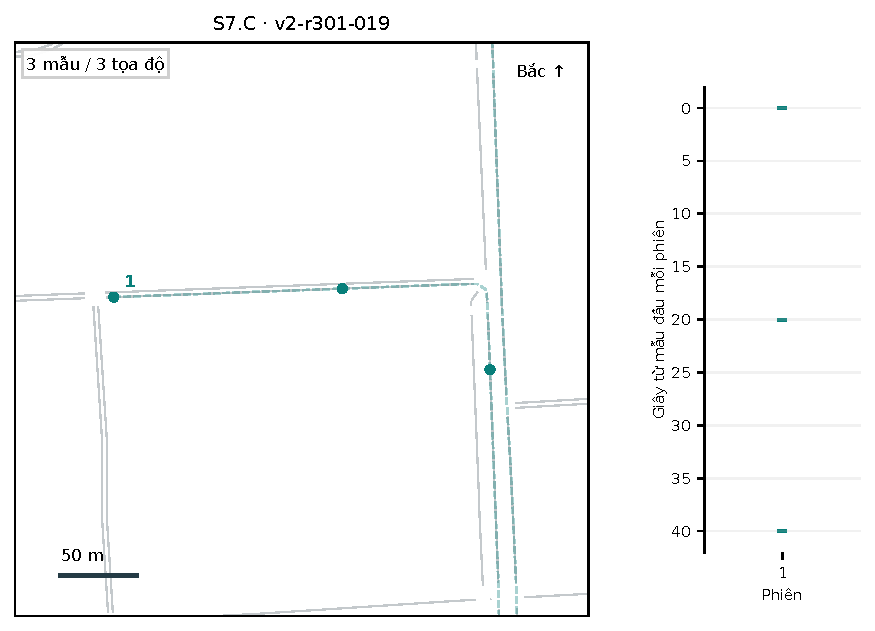
\includegraphics[width=\linewidth]{figures/case_S7_C.pdf}\end{minipage}\hfill\begin{minipage}[t]{0.42\linewidth}\vspace{0pt}\textbf{S7.C / 36 bản ghi.} Cùng truy vấn đầu nhưng chuỗi sau khác nhau; kiểm tra suy luận từ chuỗi.\par\smallskip u301\_\allowbreak{}00: 3 mẫu\par\smallskip\textbf{Đọc sample.} Ba lần query: pharmacy $\to$ clinic $\to$ hospital tại 0, 20, 40 giây. Chuỗi nội dung có thể gợi ý ý định rõ hơn một query đơn lẻ; chưa phải bằng chứng người dùng mắc bệnh.\end{minipage}\par\vspace{3pt}

\clearpage
\section{Related works gần đây: cơ chế và phạm vi}
Khảo sát tập trung vào công trình công bố trong \textbf{21/09/2023–21/09/2026}, liên quan tới công bố vị trí/quỹ đạo, nội dung, liên kết hoặc đánh giá bảo vệ. Đây là cập nhật có chọn lọc, chưa phải tổng quan hệ thống bao quát mọi paper. Mỗi nguồn được đưa vào đều có một dòng metrics ở mục sau. Liên hệ với S1–S10 là phân tích của nghiên cứu này, không phải các paper đã đánh giá đúng bộ ca A/B/C của ta.

\begingroup\small
\begin{longtable}{@{}P{3.839cm}P{6.301cm}P{6.498cm}@{}}
\toprule
\textbf{Nguồn} & \textbf{Cách tiếp cận trong 1–2 dòng} & \textbf{Liên hệ và giới hạn}\\\midrule
\endfirsthead
\toprule
\textbf{Nguồn} & \textbf{Cách tiếp cận trong 1–2 dòng} & \textbf{Liên hệ và giới hạn}\\\midrule
\endhead
\bottomrule\endfoot
TransProtect (2024) [\hyperlink{ref-R1}{R1}] & Học ngữ cảnh không gian–thời gian để tạo ứng viên; phối hợp cơ chế nhiễu/tối ưu để công bố vị trí thay thế. & Gần S1–S3; đầu ra không phải tập thật + dummy.\\
\addlinespace[3pt]
Semantic correlation (2026) [\hyperlink{ref-R2}{R2}] & Dự báo ngữ nghĩa bằng LSTM/attention, chọn dummy phù hợp chuyển tiếp đường. & S1–S3; giống ngữ nghĩa không tự bảo vệ ý định S7.\\
\addlinespace[3pt]
Fake queries (2026) [\hyperlink{ref-R3}{R3}] & Chèn truy vấn toàn giả giữa các lần truy vấn để gây khó nối đường qua thời gian. & S2–S3; cần tính toàn bộ bản tin chèn.\\
\addlinespace[3pt]
Road-aware PTPPM (2025) [\hyperlink{ref-R4}{R4}] & Cá nhân hóa nhiễu theo nhạy cảm và tương quan, dùng mạng đường để ràng buộc đầu ra. & S1–S3 và phụ thuộc thời gian; preprint, không chứng minh đã giải S5/S6 của ta.\\
\addlinespace[3pt]
CPCROK (2025) [\hyperlink{ref-R5}{R5}] & Dùng dự báo Kalman/RNN và thông điệp giả hỗ trợ đổi bí danh xe trong mạng thưa. & Liên kết xe S4; bối cảnh beacon VANET khác truy vấn POI.\\
\addlinespace[3pt]
DP-FETC (2025) [\hyperlink{ref-R6}{R6}] & Sinh quỹ đạo từ đặc trưng thống kê; xử lý điểm đầu/cuối cho quỹ đạo tương quan cao. & Gần tương quan S8 và đầu/cuối S9/S10; xuất bản ngoại tuyến.\\
\addlinespace[3pt]
Improved PIR (2025) [\hyperlink{ref-R7}{R7}] & Kết hợp truy hồi riêng tư theo từ khóa, BFV và tổ chức chỉ mục không gian. & Vị trí + nội dung S7; giao diện mã hóa khác dummy; mới xác minh tóm tắt.\\
\addlinespace[3pt]
SoK (2024) [\hyperlink{ref-R8}{R8}] & Hệ thống hóa cách kiểm tra tính hữu dụng, bảo vệ và khả năng triển khai của quỹ đạo sinh. & Cơ sở thiết kế phép đo và đối thủ; không phải đối chứng thứ bảy.\\
\addlinespace[3pt]
PRISM (2025) [\hyperlink{ref-R9}{R9}] & Dự báo LSTM kết hợp ánh xạ ngữ nghĩa phân cấp để bảo vệ chủ động. & Gợi ý xử lý ngữ cảnh/tương lai; chưa xác minh tác vụ dự đoán đích theo S6.\\
\addlinespace[3pt]
Options to Action (2026) [\hyperlink{ref-R10}{R10}] & Nghiên cứu việc sử dụng các tính năng riêng tư trên ứng dụng thể thao. & Liên quan che đầu/cuối; tỷ lệ bật tính năng không phải tỷ lệ chống tấn công.\\
\end{longtable}
\endgroup
\textbf{Đối chứng lịch sử được tách riêng.} DLS [\hyperlink{ref-B1}{B1}] và RDG [\hyperlink{ref-B2}{B2}] giữ vai trò mốc nền. AnotherMe [\hyperlink{ref-B3}{B3}] thuộc số tạp chí 2024 nhưng công bố trực tuyến 11/09/2023, sớm hơn cửa sổ 10 ngày; giữ như ngoại lệ theo yêu cầu đối chứng. Không dùng ba ngoại lệ này để chứng minh khảo sát đã cập nhật gần đây.

\textbf{Khoảng trống còn lại.} Không ép quan hệ “một scenario = một paper giải quyết trọn vẹn”. Riêng S5/S6 cần kiểm chứng đầu suy luận tương lai đúng cửa sổ; tài liệu dùng dự báo bên trong cơ chế bảo vệ chưa đủ làm bằng chứng chống suy đoán đích. S8/S9/S10 cũng phải phân biệt xuất bản ngoại tuyến với dịch vụ trực tuyến.


\clearpage
\subsection{Cơ chế liên quan trực tiếp tới S9/S10: mức phù hợp và bài học}
Bổ sung rà soát ngày 24/09/2026. “Có cơ chế cho điểm đầu/cuối” khác “đã qua benchmark A/B/C của ta”. Giữ nguồn nền ngoài ba năm khi nó trực tiếp giải bài toán; không đổi năm xuất bản hoặc gọi một chương tổng thuật là model mới.

\begingroup\small
\begin{longtable}{@{}P{3.347cm}P{6.891cm}P{6.399cm}@{}}
\toprule
\textbf{Nguồn / vai trò} & \textbf{Có thể áp dụng tới đâu?} & \textbf{Metrics / điều cần học}\\\midrule
\endfirsthead
\toprule
\textbf{Nguồn / vai trò} & \textbf{Có thể áp dụng tới đâu?} & \textbf{Metrics / điều cần học}\\\midrule
\endhead
\bottomrule\endfoot
S-TT [\hyperlink{ref-B4}{B4}]; trình bày lại [\hyperlink{ref-R11}{R11}] & Trực tiếp che địa điểm nhạy cảm ở đuôi quỹ đạo đã hoàn tất. Xét nhiều chuyến cùng đích. Đảo chiều hình học để xét đầu chuyến là phép thích nghi ngoại tuyến của ta, không phải bảo đảm online. & k-site-unidentifiability dưới tập hàm tấn công đã định; độ dài đoạn bị bỏ. Cắt tới khi tập địa điểm còn mơ hồ theo kiểm tra hướng/khoảng cách; giữ cùng tập bảo vệ qua các chuyến.\\
\addlinespace[3pt]
Endpoint Privacy Zones + đánh giá [\hyperlink{ref-B5}{B5}] & EPZ che đầu/cuối nhưng vẫn có thể bị suy từ điểm biên, mạng đường và metadata khoảng cách. Đây là nguồn tấn công/countermeasure, không phải bằng chứng EPZ đủ an toàn. & Tỷ lệ khôi phục địa điểm, độ ẩn danh hiệu dụng; kiểm tra cả metadata và nhiều hoạt động. Không gọi việc xóa tọa độ là xóa toàn bộ rò rỉ.\\
\addlinespace[3pt]
Data Stream Obfuscator [\hyperlink{ref-B6}{B6}] & Cơ chế luồng có vùng/thời gian riêng tư và cache ánh xạ nhiễu nhất quán qua các dịch vụ. Có thành phần phù hợp khi đầu/cuối nằm trong vùng/thời gian nhạy cảm; chưa xác minh kết quả trên S9/S10. & Nguồn truy cập xác nhận kiến trúc/chống trung bình nhiều bản nhiễu; chưa đủ định nghĩa metric để chép số. Học cách quản lý trạng thái và quyền phát dữ liệu nhất quán.\\
\addlinespace[3pt]
PRISM 2025 [\hyperlink{ref-R9}{R9}] & Dự đoán LSTM và ánh xạ ngữ nghĩa để xử lý điểm nhạy cảm trước khi lộ. Chỉ là thành phần có thể học cho gate; chưa xác nhận phép thử suy điểm đầu/cuối. & LPI, TDD, DC, PPT; định nghĩa đầy đủ còn cần toàn văn. Không chuyển các số cải thiện chung thành kết quả S9/S10.\\
\addlinespace[3pt]
AGeoI + dummy cho EV 2024 [\hyperlink{ref-R12}{R12}] & Bảo vệ vị trí truy vấn trạm sạc bằng nhiễu và dummy. Có thể học phần utility của truy vấn nhưng không có căn cứ coi là cơ chế che biên. & Bảo đảm approximate Geo-I và QoS trạm sạc; giao diện dịch vụ khác POI/che đầu cuối của ta.\\
\end{longtable}
\endgroup
Ưu tiên học S-TT cho tiêu chí rủi ro tại biên và EPZ cho bộ đối thủ. PRISM/AGeoI hỗ trợ thiết kế, không thay thế bằng chứng trực tiếp. Chưa thêm các nguồn này thành đối chứng thứ 7–11: sáu đối chứng chính giữ nguyên; có thể thêm S-TT ở nhánh xuất bản ngoại tuyến khi tái lập được.


\clearpage
\section{Sáu phương pháp đối chứng và điều kiện so sánh}
\begingroup\small
\begin{longtable}{@{}P{3.643cm}P{6.891cm}P{6.104cm}@{}}
\toprule
\textbf{Phương pháp} & \textbf{Backbone và đầu vào/đầu ra} & \textbf{Vai trò trong benchmark}\\\midrule
\endfirsthead
\toprule
\textbf{Phương pháp} & \textbf{Backbone và đầu vào/đầu ra} & \textbf{Vai trò trong benchmark}\\\midrule
\endhead
\bottomrule\endfoot
DLS [\hyperlink{ref-B1}{B1}] & Thống kê xác suất truy vấn/entropy; nhận vị trí hiện tại và phân bố nền, công bố tập vị trí thật + dummy. & Mốc dummy thống kê; dùng nguyên lý chọn của paper, bổ sung wrapper trạng thái nếu cần và ghi rõ.\\
\addlinespace[3pt]
RDG [\hyperlink{ref-B2}{B2}] & Thống kê chuyển tiếp, tối ưu lựa chọn dummy qua chuỗi; đầu ra các tập ứng viên theo thời gian. & Mốc có xét liên kết thời gian; Viterbi thuộc phía tấn công/đánh giá.\\
\addlinespace[3pt]
TransProtect [\hyperlink{ref-R1}{R1}] & Mô hình học sâu tạo ứng viên theo ngữ cảnh, kết hợp nhiễu/tối ưu; công bố một vị trí thay thế. & Đối chứng khác loại đầu ra; không cho đối thủ “chọn phần tử thật” trong một tập không chứa nó.\\
\addlinespace[3pt]
Semantic correlation [\hyperlink{ref-R2}{R2}] & LSTM/attention + lọc theo đường/ngữ nghĩa; công bố thật cùng K--1 dummy. & Kiểm tra ích lợi của ràng buộc ngữ nghĩa so với thống kê.\\
\addlinespace[3pt]
Fake-query insertion [\hyperlink{ref-R3}{R3}] & Quy tắc tạo/chèn truy vấn toàn giả dựa trên tính nối tiếp; transcript có thêm thời điểm/bản tin. & Giữ đúng lịch chèn; không cho đối thủ biết nhãn thật/giả nội bộ.\\
\addlinespace[3pt]
AnotherMe [\hyperlink{ref-B3}{B3}] & Hệ thống sinh quỹ đạo ảo trực tuyến, ánh xạ POI và lập tuyến; phục vụ qua vị trí/quỹ đạo thay thế. & \textbf{Đối chứng thứ sáu.} Tái lập nhánh trực tuyến hoặc gắn nhãn adapter ngoại tuyến hiện có.\\
\end{longtable}
\endgroup
\subsection{AnotherMe: sửa đúng vai trò và trạng thái}
Paper gốc mô tả hệ thống \textbf{online}; không nên gọi bản thân AnotherMe là phương pháp ngoại tuyến. Tuy nhiên adapter đang có trong repo xử lý cả đoạn/chuyến và đã được tách khỏi nhánh trực tuyến. Mục 9 đã chạy adapter này như tham chiếu offline; lỗi sinh quỹ đạo được giữ trong mẫu số utility, còn privacy chỉ tính khi có đầu ra. Mã tác giả: \url{https://github.com/fang-zhiyou/AnotherMe}.

Cần đóng gói giao diện theo tiền tố, kiểm tra đầu ra trước thời điểm t không đổi khi sửa phần tương lai, và xác định các ca áp dụng. Nếu chỉ chạy được adapter cả đoạn, báo riêng kết quả tham chiếu ngoại tuyến; không xếp chung điểm tổng với cơ chế chỉ thấy tiền tố. Khả năng áp dụng của phương pháp gốc không suy từ việc adapter hiện tại không hỗ trợ một ca.

\subsection{Sáu điều phải đồng nhất trước khi so điểm}
\begin{itemize}
\item \textbf{Đáp án:} cùng vị trí/đoạn đường/nhãn cần suy ra; không đổi tác vụ giữa các phương pháp.
\item \textbf{Đầu vào và thời gian:} cùng tiền tố, lịch sử, phụ trợ; không dùng tương lai trong nhánh trực tuyến.
\item \textbf{Đầu ra và đối thủ:} đối thủ được thiết kế theo transcript thật sự công bố, nhưng chấm cùng mục tiêu.
\item \textbf{Dịch vụ:} cùng tập POI, yêu cầu top-5, lọc trên thiết bị; ghi độ sâu phản hồi L và tất cả truy vấn phát sinh.
\item \textbf{Nguồn lực:} cùng phần cứng, ranh giới đo và ngân sách; không đồng nhất K dummy, K ứng viên nội bộ và k=5 POI.
\item \textbf{Mức tái lập:} phân biệt mã gốc, tái hiện và adaptation; báo lỗi/không áp dụng, không bỏ khỏi mẫu số để tăng điểm.
\end{itemize}
Sáu đối chứng là danh sách nghiên cứu, chưa mặc định cả sáu đều bảo vệ nội dung S7 hoặc danh tính S4. Nhánh không đổi nội dung có thể được đo như đối chứng lộ nội dung, nhưng phải trình bày đúng khả năng của nó.

Mục 9 chạy trực tiếp năm adapter trực tuyến và AnotherMe offline trên cùng dịch vụ và tập đánh giá. TransProtect dùng Markov thay Transformer; Semantic dùng bộ dự báo thực nghiệm thay LSTM. Fixed K5/K12, cache và bulk giữ vai trò kiểm tra phụ; không được đổi tên thành model từ paper. Chưa có cơ sở tuyên bố vượt cả sáu bản gốc.


\clearpage
\section{Bảng metrics gốc của toàn bộ nguồn được chọn}
Mũi tên mô tả hướng mong muốn \textbf{theo nghĩa metric gốc}. “CX” = chưa xác minh đủ trong nguồn đã truy cập, không có nghĩa paper chắc chắn không đo. Một số nguồn có vai trò khảo sát/hành vi nên không có ba cột tương đương thuật toán. Không lấy số đo trên dataset khác nhau để xếp hạng trực tiếp.

\begingroup\small
\begin{longtable}{@{}P{2.710cm}P{4.936cm}P{4.065cm}P{4.646cm}@{}}
\toprule
\textbf{Nguồn} & \textbf{Privacy / chẩn đoán} & \textbf{Utility} & \textbf{Performance / phạm vi đã kiểm tra}\\\midrule
\endfirsthead
\toprule
\textbf{Nguồn} & \textbf{Privacy / chẩn đoán} & \textbf{Utility} & \textbf{Performance / phạm vi đã kiểm tra}\\\midrule
\endhead
\bottomrule\endfoot
R1: TransProtect & EIE $\uparrow$: sai số suy luận kỳ vọng dưới đối thủ, đơn vị khoảng cách. & Sai lệch chi phí hành trình $\Delta$c $\downarrow$, so cùng đích. & CX đối với đầy đủ byte + độ trễ đầu-cuối; §5.1.4 và Eq. 13.\\
\addlinespace[3pt]
R2: Semantic & ASR $\uparrow$ theo điều kiện ẩn danh; DER $\uparrow$ đánh giá dummy/ngữ nghĩa. & DER không phải chất lượng top-5 POI. & Thời gian sinh $\downarrow$. Xem §6.3–6.5; cần khóa cách tính DER khi tái lập.\\
\addlinespace[3pt]
R3: Fake queries & Số đường khó phân biệt $\uparrow$; ASR $\uparrow$ dưới các phép loại ứng viên. & CX về chất lượng POI. & Độ trễ/tạo truy vấn và RSS $\downarrow$; §6.3–6.6.\\
\addlinespace[3pt]
R4: PTPPM & Sai số kỳ vọng của đối thủ $\uparrow$; xác suất tấn công thành công $\downarrow$. & Khoảng dịch chuyển kỳ vọng giữa thật và đầu ra $\downarrow$. & CX chi phí dịch vụ đầu-cuối; §VI, Eq. 26–27.\\
\addlinespace[3pt]
R5: CPCROK & Tỷ lệ khớp quỹ đạo của đối thủ $\rho$ $\downarrow$. & Không cùng tác vụ top-5 POI. & Số quỹ đạo giả tối thiểu $\psi$ $\downarrow$; §5.4. Đây là proxy chi phí, không phải byte.\\
\addlinespace[3pt]
R6: DP-FETC & MI $\downarrow$ giữa quỹ đạo gốc và sinh; paper trình bày bảo đảm $\varepsilon$-DP. & JSD $\downarrow$ cho phân bố vị trí, thời lượng và quãng đường. & Phân tích độ phức tạp; chưa có phép đo LBS đầu-cuối tương đương.\\
\addlinespace[3pt]
R7: Improved PIR & Phân tích an toàn; metric tấn công thực nghiệm CX. & CX metric truy hồi cụ thể. & Tóm tắt nêu tổng chi phí tính toán; đơn vị/mẫu số CX.\\
\addlinespace[3pt]
R8: SoK & Khuyến nghị kiểm tra bằng tấn công tái dựng/liên kết, bên cạnh bảo đảm hình thức. & Phân biệt metric phân bố, hình học và tác vụ downstream. & Khả năng triển khai/tính toán trong khung khảo sát; không có “điểm model SoK”.\\
\addlinespace[3pt]
R9: PRISM & Location Privacy Index (LPI); công thức CX. & Total Distance Difference; Directional Consistency; định nghĩa CX. & Privacy processing time, thời gian phản hồi; thông tin công khai, chưa tái lập.\\
\addlinespace[3pt]
R10: Adoption & Tỷ lệ dùng tính năng bảo vệ; không đo attacker success. & Nghiên cứu nhận thức/trở ngại sử dụng, không có Recall POI. & Không có chi phí thuật toán so sánh trực tiếp.\\
\addlinespace[3pt]
B1: DLS & Entropy phân bố ứng viên $\uparrow$. & CX trong hồ sơ đã kiểm tra. & CX trong hồ sơ đã kiểm tra.\\
\addlinespace[3pt]
B2: RDG & Entropy/chuyển tiếp $\uparrow$ và tỷ lệ bảo vệ dưới Viterbi $\uparrow$. & CX trong hồ sơ đã kiểm tra. & CX trong hồ sơ đã kiểm tra.\\
\addlinespace[3pt]
B3: AnotherMe & Nhận dạng quỹ đạo thật/ảo; gần mức ngẫu nhiên là mục tiêu khi tập cân bằng. & CX định nghĩa metric dịch vụ chi tiết. & Tóm tắt nêu độ trễ đáp ứng và pin; chưa xác minh đơn vị/mẫu số đầy đủ.\\
\end{longtable}
\endgroup
\subsection{Ba điểm dễ đọc nhầm}
\textbf{ASR không thống nhất giữa paper.} Ở R2, thành công là đạt điều kiện không nhận diện vị trí thật với xác suất cao hơn 1/K. R3 kiểm tra ẩn danh trước các cách khai thác khác. Không đổi tên ASR thành Hit100 hoặc dùng ASR làm “tỷ lệ tấn công thành công” mà không nêu tử số.

Riêng DER ở R2 có hai cách diễn đạt: trung bình độ tương đồng và tỷ lệ dummy đạt điều kiện. Cần xác định cách thực thi trước khi tái lập, không coi hai cách là tự động tương đương. [\hyperlink{ref-R2}{R2}]

\textbf{Dummy trông thật chưa đủ.} Nhận dạng thật/ảo của AnotherMe kiểm tra tính khó phân biệt; vẫn cần đo khả năng suy ngược vị trí thật. Tương tự, MI thấp hoặc entropy cao không tự xác nhận đối thủ cụ thể thất bại. [\hyperlink{ref-B3}{B3}, \hyperlink{ref-R6}{R6}, \hyperlink{ref-R8}{R8}]

\textbf{Chất lượng thống kê khác chất lượng dịch vụ.} JSD bảo toàn phân bố; $\Delta$c kiểm tra chi phí đến cùng đích; Recall@5 kiểm tra đúng tập POI người dùng cần. Chúng trả lời ba câu hỏi khác nhau. [\hyperlink{ref-R1}{R1}, \hyperlink{ref-R6}{R6}, \hyperlink{ref-R8}{R8}]


\clearpage
\section{Từ hạn chế metrics gốc đến bộ đo chung}
\begingroup\small
\begin{longtable}{@{}P{5.218cm}P{5.021cm}P{6.399cm}@{}}
\toprule
\textbf{Hạn chế khi dùng trực tiếp} & \textbf{Quyết định cho benchmark} & \textbf{Lập luận}\\\midrule
\endfirsthead
\toprule
\textbf{Hạn chế khi dùng trực tiếp} & \textbf{Quyết định cho benchmark} & \textbf{Lập luận}\\\midrule
\endhead
\bottomrule\endfoot
Entropy/DER/nhận dạng ảo phụ thuộc biểu diễn nội bộ. & Lấy kết quả tấn công trên đáp án thật làm privacy chính. & Một vị trí thay thế và một tập dummy đều có thể bị suy vị trí; không cần cùng cấu trúc ứng viên.\\
\addlinespace[3pt]
MAE đơn lẻ có thể bị vài sai số lớn chi phối. & MAE + median + p90; Hit50/100/200. & Vừa thấy độ lớn sai số, phân bố, vừa thấy tỷ lệ vẫn đoán rất gần.\\
\addlinespace[3pt]
Metric vị trí không chấm được người/đích/ý định. & Giữ đầu đo riêng cho từng loại đáp án. & Không ép F1, mét và entropy thành cùng một đại lượng riêng tư tự nhiên.\\
\addlinespace[3pt]
Giữ phân bố hoặc điểm thay thế gần thật chưa chứng minh POI đúng. & Recall@5, tỷ lệ trả đủ, $\Delta$D theo mạng đường. & Chấm tác vụ dịch vụ thực sự cung cấp; không chỉ chấm hình học đầu ra.\\
\addlinespace[3pt]
Số dummy hoặc thời gian sinh chưa đủ chi phí. & Byte/truy vấn thật; latency p50/p95; số bản tin phụ. & Tính cả phản hồi, truy vấn chèn và bước gộp/lọc trên thiết bị.\\
\addlinespace[3pt]
Một điểm tổng có thể che ca yếu. & Điểm tổng theo phạm vi khóa trước + bảng từng ca + ràng buộc tối thiểu. & Giữ cách lựa chọn gọn mà vẫn truy nguyên được đánh đổi.\\
\end{longtable}
\endgroup
“Bộ đo đề xuất” ở đây là \textbf{sự lựa chọn và cách vận hành hóa cho bài toán}, không tuyên bố phát minh MAE, F1, Recall hoặc trung bình nhân. Đóng góp cần chứng minh là giao thức phù hợp với threat model và phát hiện được đánh đổi mà một metric đơn lẻ bỏ qua.

\subsection{Privacy cho tọa độ: đo đối thủ, không đo khoảng cách nhiễu}
\[
e_i=d_E(x_i,\widehat x_i),\qquad \mathrm{MAE}=\frac1n\sum_i e_i,\qquad \mathrm{Hit}_r=\frac1n\sum_i\mathbf1[e_i\le r].
\]
x là vị trí thật; x̂ là ước lượng của đối thủ từ dữ liệu được phép. dE tính bằng mét sau đổi hệ tọa độ phù hợp, không lấy khoảng cách Euclid trực tiếp trên kinh/vĩ độ. MAE/median/p90 càng lớn thường càng khó định vị; Hit càng thấp càng tốt về riêng tư. Nhưng p90 cao chỉ cho biết đuôi sai số lớn, không chứng minh đa số người được bảo vệ tốt.

\textbf{Quy ước phân vị:} nearest rank, sắp e tăng dần rồi lấy e tại vị trí ceil(q$\cdot$n), tính từ 1. Với [20,50,80,150,700] m: median=80 m, p80=150 m, p90=700 m. Quy ước cố định tránh kết quả khác nhau do phần mềm nội suy.

\subsection{Privacy cho các kịch bản còn lại}
\begingroup\small
\begin{longtable}{@{}P{4.004cm}P{12.914cm}@{}}
\toprule
\textbf{Phạm vi} & \textbf{Chỉ số chính / bổ sung}\\\midrule
\endfirsthead
\toprule
\textbf{Phạm vi} & \textbf{Chỉ số chính / bổ sung}\\\midrule
\endhead
\bottomrule\endfoot
S1–S3, S9–S10 & Hit100 $\downarrow$; MAE/median/p90 $\uparrow$ và Hit50/200 $\downarrow$. S2 chấm điểm dừng; S3 chấm các thời điểm mục tiêu; S9/S10 chấm đầu/cuối.\\
\addlinespace[3pt]
S4 & Balanced accuracy $\downarrow$, precision/recall/F1 liên kết $\downarrow$; chấm người, xe, máy riêng. Mỗi đầu cần cả cặp dương và âm.\\
\addlinespace[3pt]
S5–S6 & Accuracy cạnh/đích $\downarrow$; macro-F1 nếu mất cân bằng. S6 báo thêm lỗi tọa độ; tập đích ứng viên cố định từ trước.\\
\addlinespace[3pt]
S7 & Macro-F1 ý định $\downarrow$; confusion matrix theo lớp. Tách nguyên văn và suy luận chuỗi.\\
\addlinespace[3pt]
S8 & Hit/MAE trong từng chế độ phụ trợ và chênh lệch bật–tắt; cùng tập mục tiêu, cùng đối thủ hợp lệ.\\
\end{longtable}
\endgroup
Với mọi tác vụ, thêm S(chỉ phụ trợ) và $\Delta$S = S(công bố + phụ trợ) -- S(chỉ phụ trợ), trong đó S là độ thành công của đối thủ. S5.B có thể dễ đoán ngay từ bản đồ: $\Delta$S nhỏ không đồng nghĩa mức riêng tư tuyệt đối cao.


\clearpage
\subsection{Utility: kết quả POI còn phục vụ tốt không?}
Mỗi truy vấn thật i có tập tham chiếu R* gồm tối đa 5 POI gần nhất hợp lệ của đúng loại, theo cùng oracle đường có hướng. R̂ là tối đa 5 POI sau nhận phản hồi, gộp, loại trùng và lọc trên thiết bị. L là độ sâu phản hồi của máy chủ, không phải k=5 của ứng dụng.

Trong workload hiện tại, “hợp lệ” còn yêu cầu POI đang khả dụng ở epoch của truy vấn. Tham chiếu và kết quả đều dùng cùng trạng thái server, loại POI và quy tắc xếp hạng; không chấm kết quả còn cache theo danh sách chuẩn của một thời điểm khác.

\[
\mathrm{Recall@5}_i=\frac{|R_i^\star\cap\widehat R_i|}{|R_i^\star|},\qquad C_i=\mathbf1[|\widehat R_i|=|R_i^\star|].
\]
\textbf{Ví dụ:} tham chiếu \{A,B,C,D,E\}, kết quả \{A,B,C,F,G\}: Recall=3/5=0,6 nhưng C=1 vì vẫn đủ 5. Kết quả \{A,B,C,D\}: Recall=0,8, C=0. Chỉ có đáp án tham chiếu mới vào mẫu số; có đáp án nhưng trả rỗng nhận Recall=0, C=0. Báo số truy vấn không có đáp án, không âm thầm loại bỏ lỗi dịch vụ.

\[
\Delta D_i=\frac{1}{|\widehat R_i|}\sum_{p\in\widehat R_i}d_G(Q(x_i),Q(p))-\frac{1}{|R_i^\star|}\sum_{p\in R_i^\star}d_G(Q(x_i),Q(p)).
\]
dG là đường ngắn nhất có hướng; Q ánh xạ lên mạng đường. \textbf{Cả hai vế đều xuất phát từ vị trí thật}, không so vị trí thật với vị trí giả. Chỉ chấm $\Delta$D khi trả đủ số lượng và đáp án hợp lệ, báo số ca đủ điều kiện. Nếu tham chiếu thật sự là các POI gần nhất cùng tập đủ điều kiện thì $\Delta$D $\ge$0; giá trị âm đáng kể cần kiểm tra oracle/tập lọc, không tự cắt về 0.

Ví dụ năm POI chuẩn có khoảng cách trung bình 600 m, năm POI sau bảo vệ là 850 m: $\Delta$D=250 m. Khi chỉ trả bốn POI, không gán $\Delta$D=0 để coi là tốt. Với S9/S10, lịch truy vấn thật phải được cố định trước chính sách che: truy vấn bị bỏ mà không được cache phục vụ vẫn tính là không phục vụ.

\subsection{Performance: trả giá bao nhiêu để có mức bảo vệ đó?}
\[
b=\frac{B_{\rm request}+B_{\rm response}}{N_{\rm real\ queries}},\qquad m=\frac{N_{\rm messages}}{N_{\rm real\ queries}}.
\]
\begingroup\small
\begin{longtable}{@{}P{4.305cm}P{12.614cm}@{}}
\toprule
\textbf{Đại lượng} & \textbf{Ranh giới phải ghi rõ}\\\midrule
\endfirsthead
\toprule
\textbf{Đại lượng} & \textbf{Ranh giới phải ghi rõ}\\\midrule
\endhead
\bottomrule\endfoot
b: byte/truy vấn thật $\downarrow$ & Payload tuần tự hóa thực tế của cả yêu cầu lẫn phản hồi; gồm truy vấn chèn. Nếu chỉ tính payload, ghi rõ chưa tính TLS/TCP và không gọi là lưu lượng mạng đầy đủ.\\
\addlinespace[3pt]
Thời gian p50/p95 $\downarrow$ & Từ lúc ứng dụng có truy vấn thật đến lúc có kết quả sau lọc; bao gồm sinh bảo vệ, dịch vụ và gộp. Khi dùng oracle cục bộ, báo latency cục bộ, không suy ra trải nghiệm mạng thực.\\
\addlinespace[3pt]
Chi phí chẩn đoán & Số tọa độ/bản tin, số POI phản hồi, thời gian sinh, RAM; tách học và tiền xử lý khỏi trực tuyến. Pin chỉ báo nếu đo trên thiết bị.\\
\end{longtable}
\endgroup
\key{Vòng hiện tại có byte yêu cầu/phản hồi theo schema mô phỏng, nhưng chưa có latency đầu-cuối và lưu lượng HTTP/TLS. Chưa đủ để tính điểm performance tổng hợp hoặc Q thực nghiệm mới.}

\subsection{Mẫu số và độ độc lập}
Chấm từng mục tiêu rồi gộp theo bản ghi/chuyến, nhóm tuyến, ca và scenario. Trong mỗi scenario, các ca có trọng số đều; mỗi scenario có trọng số bằng nhau. S10 dùng A/C, các scenario khác dùng A/B/C. Giữ các phiên/cặp có quan hệ trong cùng split; khoảng tin cậy lấy mẫu lại theo nhóm tuyến, không theo từng điểm FCD hoặc seed nhiễu.


\clearpage
\section{Điểm tổng hợp privacy–utility–performance}
Điểm tổng hợp phục vụ lựa chọn cấu hình trong \textbf{cùng phiên bản benchmark và cùng phạm vi}. Đây là điểm ra quyết định theo nhu cầu, không phải bảo đảm riêng tư mới hoặc xác suất an toàn. Vòng đầu chỉ xếp hạng chung S1, S2, S3, S9, S10; các giai đoạn sau mở phiên bản điểm khác.

\subsection{Bước 1: đưa ba trục về cùng chiều tốt và thang 0–1}
\[
P=1-\frac{1}{|\mathcal S|}\sum_{s\in\mathcal S}\frac1{|\mathcal C_s|}\sum_{c\in\mathcal C_s}h_{s,c},\qquad U=\operatorname{MacroMean}(\mathrm{Recall@5}).
\]
Tập ca C\_\allowbreak{}s thuộc phạm vi đã chốt: C\_\allowbreak{}10=\{A,C\}; các scenario còn lại có \{A,B,C\}. Như vậy S10 vẫn có trọng số bằng một scenario khác dù chỉ có hai ca; mẫu số không còn mặc định là 3.

h là Hit100 của đối thủ đã chọn trên validation cho từng phương pháp/ca; đóng băng lựa chọn trước test. Báo thêm envelope của các đối thủ đã thử như phân tích độ nhạy. P cao nghĩa tỷ lệ định vị đúng trong 100 m thấp. Không dùng MAE để tự co giãn theo model tốt/xấu nhất của bảng, vì thêm một model sẽ làm điểm các model cũ đổi theo.

\[
f(v;g,b)=\operatorname{clip}\!\left(\frac{b-v}{b-g},0,1\right),\quad F=\sqrt{f(b_{\rm payload};b_g,b_b)\,f(T_{95};t_g,t_b)}.
\]
Trong f, g và b là mốc tốt và mốc xấu đã chốt trước, b>g. b\_\allowbreak{}payload là byte/truy vấn thật, trung bình đều qua ca rồi scenario; T95 là giá trị lớn nhất trong các latency p95 từng ca. Như vậy một ca rất chậm không bị trung bình che lấp. Các mốc lấy từ yêu cầu dịch vụ/hardware hoặc pilot phát triển, không lấy từ test. Ở ví dụ dưới: byte tốt 2 kB, giới hạn 10 kB; latency tốt 50 ms, giới hạn 250 ms; 1 kB=1.000 byte. Đây chỉ là mốc minh họa.

\subsection{Bước 2: kiểm tra điều kiện tối thiểu rồi xếp điểm}
\[
Q=100\,P^{w_P}U^{w_U}F^{w_F},\qquad w_P,w_U,w_F>0,\quad w_P+w_U+w_F=1.
\]
Đề xuất khởi đầu wP=wU=wF=1/3. Trung bình nhân khiến một trục rất yếu kéo điểm xuống; một trục bằng 0 cho Q=0. Trước khi chọn, kiểm tra Recall@5 từng ca $\ge$0,90 và giới hạn byte/latency đã định. Cấu hình không đạt được ghi “không khả thi”, dù vẫn có thể hiển thị điểm chẩn đoán. Còn thiếu một ca bắt buộc hoặc thiếu phép đo thì Q=NA; không tự bỏ ca rồi chia lại trọng số.

\subsection{Ví dụ số — dữ liệu minh họa, không phải kết quả model}
\begingroup\small
\begin{longtable}{@{}P{2.188cm}P{2.854cm}P{4.946cm}P{2.758cm}P{3.329cm}@{}}
\toprule
\textbf{Cấu hình} & \textbf{P / U} & \textbf{Byte; latency p95} & \textbf{F} & \textbf{Q đều}\\\midrule
\endfirsthead
\toprule
\textbf{Cấu hình} & \textbf{P / U} & \textbf{Byte; latency p95} & \textbf{F} & \textbf{Q đều}\\\midrule
\endhead
\bottomrule\endfoot
M1 & 0.95 / 0.95 & 6,800 B; 130 ms & 0.490 & 76.2\\
\addlinespace[3pt]
M2 & 0.70 / 0.95 & 3,600 B; 90 ms & 0.800 & 81.0\\
\end{longtable}
\endgroup
M1/M2 là hai cấu hình giả định, không phải kết quả thực nghiệm. M1 có privacy tốt hơn, M2 có chi phí thấp hơn; Q phản ánh bộ trọng số đang dùng. Utility trung bình 0,95 chưa đủ chứng minh mọi ca đạt 0,90; ví dụ giả định đã qua kiểm tra từng ca.


\clearpage
\subsection{Trọng số thay đổi thì quyết định có đổi không?}
\begingroup\small
\begin{longtable}{@{}P{7.646cm}P{2.516cm}P{2.516cm}P{3.678cm}@{}}
\toprule
\textbf{Ưu tiên (wP, wU, wF)} & \textbf{Q của M1} & \textbf{Q của M2} & \textbf{Thứ tự}\\\midrule
\endfirsthead
\toprule
\textbf{Ưu tiên (wP, wU, wF)} & \textbf{Q của M1} & \textbf{Q của M2} & \textbf{Thứ tự}\\\midrule
\endhead
\bottomrule\endfoot
Cân bằng (1/3, 1/3, 1/3) & 76.2 & 81.0 & M2 > M1\\
\addlinespace[3pt]
Ưu tiên privacy (0,6; 0,2; 0,2) & 83.2 & 76.4 & M1 > M2\\
\addlinespace[3pt]
Ưu tiên performance (0,2; 0,2; 0,6) & 63.8 & 80.6 & M2 > M1\\
\end{longtable}
\endgroup
Đây là đổi nhu cầu hợp lệ, không phải thay công thức sau khi thấy model nào thắng. Cần công bố hồ sơ trọng số chính trước test và giữ các hồ sơ còn lại làm phân tích độ nhạy. Thực nghiệm phải báo đủ P, U, F, Q, điều kiện khả thi và kết quả từng ca.

\subsection{Mở rộng điểm sang S5/S6/S8 rồi S4/S7}
Giai đoạn II bổ sung độ đúng cạnh/đích và chế độ có phụ trợ; giai đoạn III bổ sung liên kết và ý định. Khi đó có thể chọn một đại lượng thành công của đối thủ cho từng đầu để tính 1--S, nhưng \textbf{không được coi 1--accuracy, 1--F1 và 1--Hit là cùng mức riêng tư tự nhiên}. Số lớp, tỷ lệ cặp dương, tập ứng viên và mức đoán nền phải được cố định. Chỉ tạo Q đa nhiệm khi đã chốt trọng số tác vụ và phép chuẩn hóa tương ứng; hiện chưa có Q chung S1–S10.

S8 cần báo cả mức rủi ro tuyệt đối khi có phụ trợ và phần tăng thêm. S4 phải có ba đầu người/xe/máy; hiện còn thiếu nhãn/độ cân bằng nên chưa đủ điều kiện tạo điểm. Không gán các phần chưa đo bằng 0 hay dùng “không áp dụng” như điểm hoàn hảo.

\key{Chấp nhận một điểm kết hợp ba trục, nhưng luôn gắn với phạm vi, trọng số và điều kiện áp dụng. Không có một con số duy nhất thay thế toàn bộ phân tích S1–S10.}

\subsection{Quy trình đánh giá đề xuất cho vòng tiếp theo}
\begin{itemize}
\item Khóa phiên bản dataset, oracle POI, các cửa sổ, tập nhãn và quyền phụ trợ; ghi hash nguồn.
\item Tách dữ liệu học, chọn cấu hình và xác nhận theo nhóm quan hệ. Dữ liệu từng dùng để chỉnh thiết kế không còn là kiểm thử mới.
\item Học/chọn đối thủ trên phần được phép; chọn cấu hình bảo vệ và trọng số trên phát triển/validation, rồi đóng băng.
\item Chạy toàn bộ cấu hình đã đăng ký, cùng seed nhiễu ghép cặp; giữ lỗi và ca thiếu, ghi nguyên nhân.
\item Báo từng ca, từng nhóm, ba trục và điểm Q; khoảng tin cậy theo nhóm tuyến. Test dùng để kết luận, không để tiếp tục tối ưu.
\end{itemize}
Trong bộ minh họa thuộc phạm vi hiện tại, S5.C và S6.A có 4 bản ghi, S6.B có 5. Mỗi bộ thực nghiệm có mẫu số riêng. Cần tăng nhóm độc lập theo điều kiện cố định; thêm cửa sổ từ cùng chuyến không khắc phục được thiếu độc lập.


\clearpage
\section{Phương pháp truy vấn công khai theo loại POI}
\textbf{Mục tiêu:} tìm top-5 POI đang khả dụng gần người dùng theo đường có hướng. Thiết bị có mạng đường và danh mục 419 POI; máy chủ giữ trạng thái khả dụng. Cơ chế chọn trước tập truy vấn từ dữ liệu công khai; GPS thật chỉ dùng để xếp hạng kết quả tại thiết bị.

\begin{center}
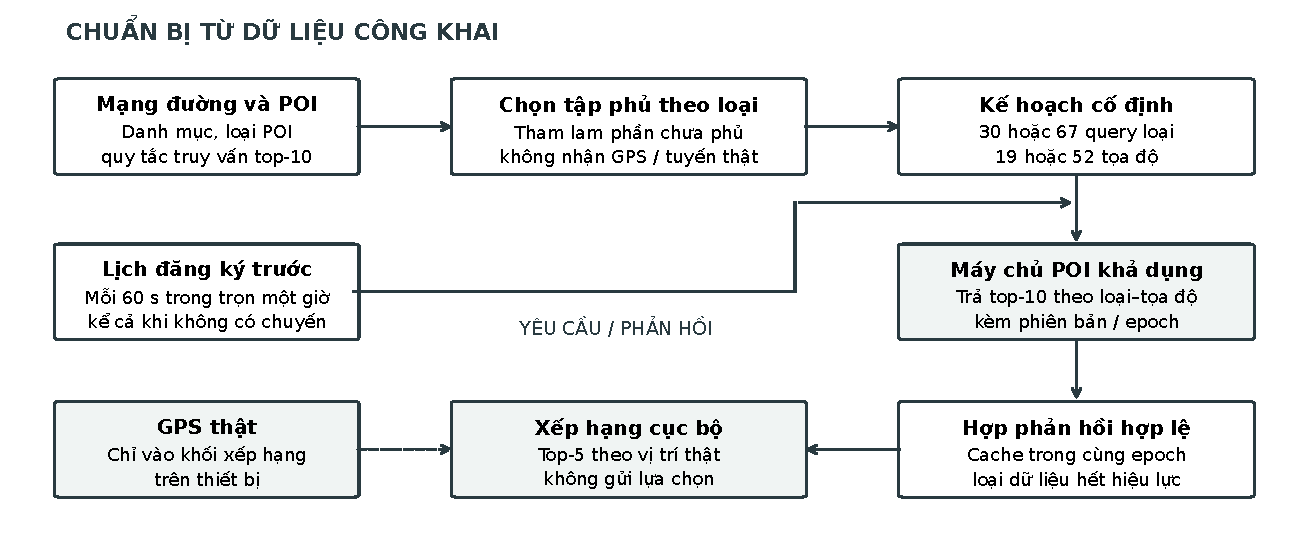
\includegraphics[width=\linewidth]{figures/architecture_current.pdf}
\end{center}
Hình. Kế hoạch truy vấn dùng chung cho mọi người trong vùng đã xác định. Máy chủ trả các POI khả dụng; thiết bị hợp phản hồi hợp lệ và dùng GPS thật để chọn kết quả, không gửi lựa chọn đó ra ngoài.

\subsection{Chọn tập truy vấn theo độ phủ danh mục}
Với mỗi loại, dựng top-10 tĩnh tại các tọa độ ứng viên trên mạng đường. Mỗi bước chọn truy vấn bổ sung tỷ lệ POI chưa phủ lớn nhất của một loại; tọa độ phải qua đúng quy tắc server ánh xạ lên đường. Đây là tối ưu tham lam từ danh mục công khai, không phải deep learning hay một cơ chế nhiễu epsilon.

\[
(c^*,v^*)=\arg\max_{c,v}\frac{|\mathcal P_{10,c}(v)\setminus U_c|}{|\mathcal P_c|},\qquad U_{c^*}\leftarrow U_{c^*}\cup\mathcal P_{10,c^*}(v^*).
\]
Tử số đếm POI mới do truy vấn bổ sung; mẫu số là tổng POI của loại đang xét. U là tập POI đã phủ của từng loại, được cập nhật sau mỗi lựa chọn.

\begingroup\small
\begin{longtable}{@{}P{3.347cm}P{6.891cm}P{6.399cm}@{}}
\toprule
\textbf{Cấu hình} & \textbf{Quy tắc dừng và phân bổ} & \textbf{Giao diện mỗi lần tải}\\\midrule
\endfirsthead
\toprule
\textbf{Cấu hình} & \textbf{Quy tắc dừng và phân bổ} & \textbf{Giao diện mỗi lần tải}\\\midrule
\endhead
\bottomrule\endfoot
30 truy vấn & Dừng ở 30: cà phê 11; phòng khám 1; trạm xăng 1; bệnh viện 1; nhà thuốc 2; nhà hàng 14. & 30 truy vấn loại–tọa độ, tại 19 tọa độ khác nhau.\\
\addlinespace[3pt]
67 truy vấn: phủ rộng & Tiếp tục đến khi không tăng độ phủ tĩnh; tổng 67 truy vấn. & 67 truy vấn loại–tọa độ, tại 52 tọa độ khác nhau.\\
\end{longtable}
\endgroup
Mỗi tọa độ được giữ cố định; các loại không buộc dùng chung một tập vị trí. Thiết bị hỏi theo kế hoạch đã khóa, không chọn query từ GPS, tuyến tương lai hoặc trạng thái khả dụng thật. So sánh phải đếm riêng truy vấn loại, tọa độ và byte.


\clearpage
\subsection{Lập luận privacy cho S1/S2/S3/S9 và S10.A/C}
Gọi X là hành trình, A là giờ sử dụng riêng tư; C gồm vùng, danh mục, kế hoạch và khoảng đăng ký công khai; W là trạng thái server; T là transcript yêu cầu/phản hồi. Client gửi mỗi 60 giây trong trọn khoảng [0, 3600), kể cả trước/sau chuyến hoặc không dùng dịch vụ; đọc cache không kích hoạt bản tin. Với C được chốt trước hoạt động:

\[
T=f(C,W)\quad\Longrightarrow\quad I((X,A);T\mid C,W)=0.
\]
\begingroup\small
\begin{longtable}{@{}P{4.505cm}P{12.414cm}@{}}
\toprule
\textbf{Mục tiêu cần bảo vệ} & \textbf{Vì sao tọa độ công bố không bổ sung thông tin}\\\midrule
\endfirsthead
\toprule
\textbf{Mục tiêu cần bảo vệ} & \textbf{Vì sao tọa độ công bố không bổ sung thông tin}\\\midrule
\endhead
\bottomrule\endfoot
S1: vị trí hiện tại & Ở vị trí nào trong cùng vùng, client cũng gửi cùng kế hoạch.\\
\addlinespace[3pt]
S2: nơi dừng & Tọa độ không tập trung quanh nơi dừng; lịch vẫn chạy khi không có hoạt động.\\
\addlinespace[3pt]
S3: đoạn đường đã đi & Chuỗi tọa độ cố định không bám đường đi thật.\\
\addlinespace[3pt]
S9; S10.A/C: đầu/cuối & Tọa độ không chọn từ endpoint; giờ bắt đầu/kết thúc chuyến không điều khiển lịch gửi trong khoảng đăng ký.\\
\end{longtable}
\endgroup
\key{Bảo vệ payload và giờ gửi trong khoảng công khai; prior vẫn có thể giúp đối thủ đoán. Không gán Hit=0 hoặc MAE vô hạn từ công thức trên.}

Điều kiện: đăng ký khoảng cố định trước chuyến, không hủy sớm hay đổi vùng/kế hoạch theo GPS. Account, IP, click và lỗi mạng nằm ngoài bảo đảm. Sáu kiểm tra trên server mô phỏng đối chiếu lịch đọc sớm/muộn/không đọc cho cùng yêu cầu và phản hồi. Đây là kiểm tra cơ chế, không chứng minh mọi kênh mạng đã an toàn.

\subsection{Lập luận utility và hiệu lực phản hồi}
Một POI thuộc top-10 tĩnh vẫn thuộc top-10 sống nếu chính nó khả dụng: loại các POI không khả dụng không làm nó tụt hạng. Nếu hợp truy vấn phủ mọi POI có thể tới được, hợp phản hồi chứa đủ POI để phục hồi top-5 thật. Điều kiện gồm cùng khoảng cách đường, quy tắc phá hòa và phản hồi hợp lệ.

Trên mạng đang dùng, cấu hình 30 còn \textbf{160 POI}, cấu hình 67 còn \textbf{8 POI} ngoài hợp phủ tĩnh. Tọa độ ứng viên thuộc thành phần liên thông mạnh lớn nhất, còn tập đích xét toàn danh mục đường. Vì vậy, 100\% trên các ca đã thử chưa phải chứng nhận toàn bản đồ.

Server giữ trạng thái trong epoch 60 giây; client chỉ dùng phản hồi còn hiệu lực. Bảng mục 9 là kiểm tra trên bốn nhóm, gửi mỗi sự kiện. Mục 10 dùng 32 nhóm mới và client theo lịch công khai; tính cả bản tin ngoài thời gian hoạt động. Ablation so với cùng kế hoạch chỉ refresh trong epoch có hoạt động để đo đúng giá của việc che giờ bắt đầu/kết thúc.


\clearpage
\section{Đối chứng trực tiếp trên cùng dịch vụ}
Bảng chính so phương pháp đề xuất với \textbf{DLS, RDG, TransProtect, Semantic correlation, Fake-query insertion và AnotherMe}. Các số dưới được chạy lại trong cùng bộ đánh giá. Đây là các bản thích nghi có mô tả mã và giả định; không phải số chép từ paper hoặc chứng nhận tái lập đầy đủ.

Cùng OSM/SUMO, 419 POI, sáu loại; server trả top-10 khả dụng, thiết bị chọn top-5 theo đường. Trạng thái đổi theo epoch 60 giây; thử p=0,5/0,8/0,95 và ba world seed. Tất cả được hợp phản hồi còn hiệu lực. Bảng này gửi ở mọi sự kiện, chưa che giờ hoạt động; đếm cả query giả và byte JSON thực. Client theo lịch công khai được đo riêng ở mục 10.

Fit thống kê/attacker trên nhóm 501–502; chọn attacker trên 601–602. Phạm vi 14 ca giữ 165 record từ 94 chuyến của 12 nhóm phát triển và 54 record từ 30 chuyến của bốn nhóm 901–904. Các số được tổng hợp lại từ kết quả cố định; không huấn luyện/chọn attacker mới. Đây là đối chứng phát triển, chưa phải xác nhận độc lập mới.

\subsection{Kết quả chính trên bốn nhóm 901–904, p=0,8}
\begingroup\small
\begin{longtable}{@{}P{3.469cm}P{2.282cm}P{1.643cm}P{2.921cm}P{3.104cm}P{2.374cm}@{}}
\toprule
\textbf{Phương pháp} & \textbf{Recall@5 $\uparrow$} & \textbf{Ca $\ge$90\%} & \textbf{Byte / yêu cầu thật $\downarrow$} & \textbf{Sinh tọa độ: ms / yêu cầu $\downarrow$} & \textbf{Lượt record hợp lệ}\\\midrule
\endfirsthead
\toprule
\textbf{Phương pháp} & \textbf{Recall@5 $\uparrow$} & \textbf{Ca $\ge$90\%} & \textbf{Byte / yêu cầu thật $\downarrow$} & \textbf{Sinh tọa độ: ms / yêu cầu $\downarrow$} & \textbf{Lượt record hợp lệ}\\\midrule
\endhead
\bottomrule\endfoot
Vị trí thật & 100,00\% & 14/14 & 242,8 & <0,001 & 108/108\\
\addlinespace[3pt]
DLS & 100,00\% & 14/14 & 962,7 & 0,423 & 108/108\\
\addlinespace[3pt]
RDG & 100,00\% & 14/14 & 950,7 & 1,407 & 108/108\\
\addlinespace[3pt]
TransProtect* & 99,69\% & 14/14 & 242,7 & 5,532 & 108/108\\
\addlinespace[3pt]
Semantic* & 100,00\% & 14/14 & 967,4 & 1,062 & 108/108\\
\addlinespace[3pt]
Fake-query* & 100,00\% & 14/14 & 1313,2 & 0,756 & 108/108\\
\addlinespace[3pt]
AnotherMe† & 17,37\% & 0/14 & 241,7 & 1,858 & 30/108\\
\addlinespace[3pt]
Đề xuất 30 & 94,75\% & 14/14 & 2389,7 & <0,001 & 108/108\\
\addlinespace[3pt]
Đề xuất 67 & 100,00\% & 14/14 & 5353,9 & <0,001 & 108/108\\
\end{longtable}
\endgroup
Lượt record = record $\times$ hai seed; có thể dùng chung chuyến. Chi phí tính trên các chuyến còn thuộc phạm vi, giữ toàn bộ clock và bản tin gốc của mỗi chuyến; chưa gồm HTTP/TLS. Thời gian là tính toán Python, không gồm server/RTT hoặc chuẩn bị model. Chi phí AnotherMe chỉ trên phiên sinh thành công; không xếp hạng với phương pháp trực tuyến.

\textbf{Giữ đúng đầu ra:} DLS/RDG/Semantic gửi tập có vị trí thật; TransProtect/AnotherMe trả vị trí thay thế; Fake-query thêm thời điểm gửi. Đề xuất 30/67 dùng 19/52 tọa độ. Cùng dịch vụ không có nghĩa cùng byte, cùng số tọa độ hoặc cùng bảo đảm privacy.

\key{Fixed K5/K12 và bulk là phép kiểm tra thiết kế phụ. Chúng không thay thế sáu đối chứng nghiên cứu trong bảng chính.}


\clearpage
\subsection{Privacy: suy luận đúng trong bán kính 100 m}
Mỗi ô là \textbf{Hit100 $\downarrow$ / MAE (m) $\uparrow$}, trung bình đều các ca: S10 dùng A/C, các scenario khác dùng A/B/C. Gộp seed trong record rồi nhóm. MAE và Hit chọn decoder riêng trên tập chọn attacker. Đối thủ chỉ thấy tọa độ, thời gian tương đối và liên kết được phép; không thấy nhãn thật/giả hoặc đáp án.

\begingroup\small
\begin{longtable}{@{}P{3.469cm}P{2.465cm}P{2.465cm}P{2.465cm}P{2.465cm}P{2.465cm}@{}}
\toprule
\textbf{Phương pháp} & \textbf{S1} & \textbf{S2} & \textbf{S3} & \textbf{S9} & \textbf{S10}\\\midrule
\endfirsthead
\toprule
\textbf{Phương pháp} & \textbf{S1} & \textbf{S2} & \textbf{S3} & \textbf{S9} & \textbf{S10}\\\midrule
\endhead
\bottomrule\endfoot
Vị trí thật & 100,00\% / 5 & 100,00\% / 6 & 100,00\% / 4 & 16,67\% / 207 & 12,50\% / 430\\
\addlinespace[3pt]
DLS & 50,00\% / 1400 & 41,67\% / 1613 & 95,76\% / 93 & 8,33\% / 1042 & 12,50\% / 413\\
\addlinespace[3pt]
RDG & 58,33\% / 1771 & 62,50\% / 755 & 95,83\% / 59 & 4,17\% / 1484 & 12,50\% / 2104\\
\addlinespace[3pt]
TransProtect* & 66,67\% / 101 & 79,17\% / 50 & 74,59\% / 83 & 18,75\% / 219 & 12,50\% / 395\\
\addlinespace[3pt]
Semantic* & 83,33\% / 59 & 100,00\% / 13 & 84,39\% / 42 & 33,33\% / 312 & 0,00\% / 515\\
\addlinespace[3pt]
Fake-query* & 50,00\% / 1536 & 33,33\% / 1489 & 96,91\% / 47 & 12,50\% / 483 & 6,25\% / 393\\
\addlinespace[3pt]
AnotherMe† & 0,00\% / 1697 & — / — & 0,00\% / 1877 & 0,00\% / 1565 & 0,00\% / 1914\\
\addlinespace[3pt]
Đề xuất 30 & 0,00\% / 2104 & 0,00\% / 2055 & 0,00\% / 2068 & 0,00\% / 2618 & 0,00\% / 2156\\
\addlinespace[3pt]
Đề xuất 67 & 0,00\% / 2104 & 0,00\% / 1859 & 0,00\% / 2068 & 0,00\% / 2488 & 0,00\% / 2238\\
\end{longtable}
\endgroup
Bộ đối thủ gồm thống kê tập điểm, prior, Viterbi, ngoại suy 30/60/120 giây, kNN và Extra Trees; chọn bằng nhóm 601–602. AnotherMe chỉ gộp ca có đầu ra: S1 thiếu C; S2 thiếu cả ba; S9 thiếu B; S10 chỉ có C. Không so các ô này như cùng mẫu số. Chi tiết 14 ca: active\_\allowbreak{}scope\_\allowbreak{}ac\_\allowbreak{}v2/readout.json.

\textbf{Phép thử bốn nhóm này:} S10.A/C của vị trí thật đạt Hit100 12,50\%, A là 0\%, C là 25\%. S9 chỉ B có hit. Bằng chứng endpoint ở đây chủ yếu từ S9.B/S10.C. Mục 10 dùng bộ suy luận đường mạnh hơn và 32 nhóm để kiểm tra S9, S10.A/C; không trộn hai bộ số.

Hit bằng 0 chỉ là không trúng trong các mẫu và bộ attacker đã thử. Vùng dịch vụ, lịch mở/đóng ứng dụng, account, IP và click chưa được bảo vệ toàn diện. Lập luận tọa độ độc lập GPS ở mục 8 vẫn có điều kiện; không thay thế bằng chứng tấn công thực nghiệm.

\subsection{Bản triển khai được so sánh là gì?}
\begingroup\small
\begin{longtable}{@{}P{3.804cm}P{13.115cm}@{}}
\toprule
\textbf{Đối chứng} & \textbf{Thành phần chạy và giới hạn}\\\midrule
\endfirsthead
\toprule
\textbf{Đối chứng} & \textbf{Thành phần chạy và giới hạn}\\\midrule
\endhead
\bottomrule\endfoot
DLS / RDG & DLS chọn theo entropy; RDG dùng pool DLS và entropy của trọng số max-product. Thống kê từ background SUMO; trạng thái đường thay ô lưới paper.\\
\addlinespace[3pt]
TransProtect* & Lõi chọn ứng viên + nhiễu của paper; bộ dự báo Markov thay Transformer chưa có checkpoint tác giả. Không diễn giải là đã vượt model deep learning gốc.\\
\addlinespace[3pt]
Semantic* & Bộ chọn theo ngữ nghĩa/chuyển tiếp; nhãn POI OSM và dự báo thực nghiệm thay dữ liệu AMap/LSTM chưa có weights.\\
\addlinespace[3pt]
Fake-query* & Có chèn thật các bản tin toàn giả, lọc chuyển động theo đường và fallback DLS. Phân bố thời gian, lịch sử và ngưỡng là giả định công khai của adapter.\\
\addlinespace[3pt]
AnotherMe† & Chạy VTGA với ánh xạ/lập tuyến nội bộ. Đọc cả chuyến nên chỉ là tham chiếu offline; mẫu quá ngắn không bị kéo giãn để tạo kết quả hợp lệ.\\
\end{longtable}
\endgroup

\clearpage
\subsection{Đủ 14 ca hiện tại: utility và tỷ lệ chạy thành công}
Recall@5 ở p=0,8 trên cùng bốn nhóm; \textbf{† là tham chiếu offline}. Trong bảng này, nếu record thiếu đầu ra của một phiên, mọi yêu cầu có đáp án trong record nhận Recall=0; yêu cầu không có POI tham chiếu giữ null. Privacy thiếu đầu ra để trống. Mục 10 báo riêng giao thức tính lỗi theo từng yêu cầu/phiên.

\begingroup\small
\begin{longtable}{@{}P{1.269cm}P{1.450cm}P{1.450cm}P{1.722cm}P{1.812cm}P{1.540cm}P{1.722cm}P{1.993cm}P{1.993cm}@{}}
\toprule
\textbf{Ca} & \textbf{DLS} & \textbf{RDG} & \textbf{Trans.*} & \textbf{Semantic*} & \textbf{Fake*} & \textbf{Another†} & \textbf{Đề xuất 30} & \textbf{Đề xuất 67}\\\midrule
\endfirsthead
\toprule
\textbf{Ca} & \textbf{DLS} & \textbf{RDG} & \textbf{Trans.*} & \textbf{Semantic*} & \textbf{Fake*} & \textbf{Another†} & \textbf{Đề xuất 30} & \textbf{Đề xuất 67}\\\midrule
\endhead
\bottomrule\endfoot
S1.A & 100,00\% & 100,00\% & 99,83\% & 100,00\% & 100,00\% & 33,61\% & 95,17\% & 100,00\%\\
\addlinespace[3pt]
S1.B & 100,00\% & 100,00\% & 100,00\% & 100,00\% & 100,00\% & 33,61\% & 98,28\% & 100,00\%\\
\addlinespace[3pt]
S1.C & 100,00\% & 100,00\% & 99,86\% & 100,00\% & 100,00\% & 0,00\% & 96,83\% & 100,00\%\\
\addlinespace[3pt]
S2.A & 100,00\% & 100,00\% & 100,00\% & 100,00\% & 100,00\% & 0,00\% & 90,15\% & 100,00\%\\
\addlinespace[3pt]
S2.B & 100,00\% & 100,00\% & 100,00\% & 100,00\% & 100,00\% & 0,00\% & 90,78\% & 100,00\%\\
\addlinespace[3pt]
S2.C & 100,00\% & 100,00\% & 100,00\% & 100,00\% & 100,00\% & 0,00\% & 91,29\% & 100,00\%\\
\addlinespace[3pt]
S3.A & 100,00\% & 100,00\% & 99,76\% & 100,00\% & 100,00\% & 33,02\% & 96,50\% & 100,00\%\\
\addlinespace[3pt]
S3.B & 100,00\% & 100,00\% & 99,80\% & 100,00\% & 100,00\% & 33,02\% & 95,87\% & 100,00\%\\
\addlinespace[3pt]
S3.C & 100,00\% & 100,00\% & 99,29\% & 100,00\% & 100,00\% & 32,94\% & 96,46\% & 100,00\%\\
\addlinespace[3pt]
S9.A & 100,00\% & 100,00\% & 99,24\% & 100,00\% & 100,00\% & 33,08\% & 95,78\% & 100,00\%\\
\addlinespace[3pt]
S9.B & 100,00\% & 100,00\% & 99,30\% & 100,00\% & 100,00\% & 0,00\% & 95,45\% & 100,00\%\\
\addlinespace[3pt]
S9.C & 100,00\% & 100,00\% & 99,53\% & 100,00\% & 100,00\% & 24,65\% & 95,85\% & 100,00\%\\
\addlinespace[3pt]
S10.A & 100,00\% & 100,00\% & 99,59\% & 100,00\% & 100,00\% & 0,00\% & 93,68\% & 100,00\%\\
\addlinespace[3pt]
S10.C & 100,00\% & 100,00\% & 99,53\% & 100,00\% & 100,00\% & 24,45\% & 94,83\% & 100,00\%\\
\end{longtable}
\endgroup
\subsection{Đóng góp được hỗ trợ tới đâu trên năm scenario?}
\begingroup\small
\begin{longtable}{@{}P{2.560cm}P{6.596cm}P{7.482cm}@{}}
\toprule
\textbf{Scenario} & \textbf{Hit100: năm adapter $\to$ đề xuất} & \textbf{Mức bằng chứng}\\\midrule
\endfirsthead
\toprule
\textbf{Scenario} & \textbf{Hit100: năm adapter $\to$ đề xuất} & \textbf{Mức bằng chứng}\\\midrule
\endhead
\bottomrule\endfoot
S1 & 50,00\%–83,33\% $\to$ 0\% & 4 nhóm; kế hoạch mỗi sự kiện\\
\addlinespace[3pt]
S2 & 33,33\%–100,00\% $\to$ 0\% & 4 nhóm; kế hoạch mỗi sự kiện\\
\addlinespace[3pt]
S3 & 74,59\%–96,91\% $\to$ 0\% & 4 nhóm; kế hoạch mỗi sự kiện\\
\addlinespace[3pt]
S9 & 19,76\%–40,81\% $\to$ 0\% & 32 nhóm; kế hoạch theo lịch\\
\addlinespace[3pt]
S10 (A/C) & 10,75\%–26,11\% $\to$ 0\% & 32 nhóm; kế hoạch theo lịch\\
\end{longtable}
\endgroup
\textbf{Đóng góp hiện có:} phối hợp chọn truy vấn theo độ phủ POI, xếp hạng GPS tại thiết bị và lịch công khai để giảm lộ vị trí/đường/endpoint trong dịch vụ trạng thái động. Đã có lợi thế thực nghiệm ở cả năm scenario; lịch được kiểm tra riêng về giờ hoạt động. S1–S3 cần chạy lại privacy trên cohort lớn; chưa gán số bốn nhóm cho phiên bản theo lịch.

Đây là đóng góp thiết kế và đánh giá trong phạm vi đã định. Chi phí truyền cao hơn; chưa chứng minh mới so với toàn bộ tài liệu, vượt sáu model gốc hoặc tối ưu ở cùng byte/latency. AnotherMe là tham chiếu offline với mẫu số khác.


\clearpage
\section{S9 và S10.A/C trên 32 nhóm tuyến}
\textbf{Cohort dựng sau khi khóa kế hoạch và attacker:} đủ 32 seed, 704 chuyến. Phạm vi hiện tại giữ 1093/1118 record gốc; utility năm scenario dùng 435 record từ 246 chuyến, privacy S9/S10 dùng 150. Không gộp pilot bảy nhóm. Trùng nguyên tuyến với tập phát triển/pilot: 0/0; vẫn cùng thành phố và bộ sinh SUMO. Thu hẹp S10 sau chẩn đoán; đây là tổng hợp lại, không phải đợt test mới.

Giữ bank cũ; thêm suy luận xuôi/ngược theo \textbf{mạng đường có hướng}, vận tốc quan sát và nhiều horizon; ca C kết hợp chuyến liên kết. Fit/chọn trên 10/10 nhóm khác; giữ nguyên lựa chọn cho 32 nhóm mới. Đối thủ không nhận đoạn bị giấu, endpoint thật hoặc thời gian cắt thật.

Mỗi ô privacy là \textbf{Hit100 $\downarrow$ / MAE (m) $\uparrow$}: S9 gộp A/B/C, S10 gộp A/C. Recall gộp 14 ca rồi đều qua năm scenario ở p=0,8. Chi phí chỉ trên chuyến được giữ, gồm toàn clock gốc và cả giờ cover traffic; chưa có HTTP/TLS. Đây không phải so ở cùng byte.

\begingroup\small
\begin{longtable}{@{}P{3.900cm}P{3.329cm}P{3.329cm}P{2.663cm}P{2.854cm}@{}}
\toprule
\textbf{Phương pháp} & \textbf{S9: Hit / MAE} & \textbf{S10.A/C: Hit / MAE} & \textbf{Recall@5 $\uparrow$} & \textbf{Byte $\downarrow$}\\\midrule
\endfirsthead
\toprule
\textbf{Phương pháp} & \textbf{S9: Hit / MAE} & \textbf{S10.A/C: Hit / MAE} & \textbf{Recall@5 $\uparrow$} & \textbf{Byte $\downarrow$}\\\midrule
\endhead
\bottomrule\endfoot
Vị trí thật & 42,5\% / 165 & 17,4\% / 212 & 100,0\% & 250\\
\addlinespace[3pt]
DLS & 34,3\% / 462 & 11,2\% / 222 & 100,0\% & 952\\
\addlinespace[3pt]
RDG & 19,8\% / 793 & 10,7\% / 224 & 100,0\% & 944\\
\addlinespace[3pt]
TransProtect* & 33,6\% / 243 & 13,3\% / 259 & 99,7\% & 250\\
\addlinespace[3pt]
Semantic* & 40,8\% / 184 & 11,8\% / 292 & 100,0\% & 976\\
\addlinespace[3pt]
Fake-query* & 31,4\% / 522 & 26,1\% / 213 & 100,0\% & 1296\\
\addlinespace[3pt]
AnotherMe† & 0,0\% / 1687 & 0,0\% / 1232 & 16,8\% & 239\\
\addlinespace[3pt]
Đề xuất 30 + lịch & 0,0\% / 2232 & 0,0\% / 1916 & 95,0\% & 3071\\
\addlinespace[3pt]
Đề xuất 67 + lịch & 0,0\% / 2311 & 0,0\% / 1916 & 100,0\% & 6879\\
\end{longtable}
\endgroup
* Giữ giới hạn adapter ở mục 9. † AnotherMe offline: privacy chỉ trên tập con thành công; utility giữ yêu cầu lỗi bằng 0. Stress p=0,95: đề xuất 30 đạt 93,0\%, 13/14 ca $\ge$90\%; bản 67 đạt 100,0\%.

\subsection{Control theo ca: không phải mọi Hit=0 đều có sức phân biệt}
\begingroup\small
\begin{longtable}{@{}P{2.420cm}P{4.065cm}P{4.549cm}P{5.323cm}@{}}
\toprule
\textbf{Ca / nhóm} & \textbf{Raw: Hit100 / Hit200} & \textbf{67 + lịch: Hit100 / Hit200} & \textbf{MAE raw $\to$ đề xuất (m)}\\\midrule
\endfirsthead
\toprule
\textbf{Ca / nhóm} & \textbf{Raw: Hit100 / Hit200} & \textbf{67 + lịch: Hit100 / Hit200} & \textbf{MAE raw $\to$ đề xuất (m)}\\\midrule
\endhead
\bottomrule\endfoot
S10.A / 31 & 12,9\% / 35,5\% & 0,0\% / 0,0\% & 204 $\to$ 1914\\
\addlinespace[3pt]
S10.C / 32 & 21,9\% / 46,9\% & 0,0\% / 0,0\% & 219 $\to$ 1919\\
\end{longtable}
\endgroup
\textbf{Lợi thế trong phạm vi hiện tại:} Hit100 S10.A/C của năm adapter là 10,75–26,11\%, lịch công khai 0\%. Raw control có hit ở cả A/C nên các ca có khả năng phân biệt. Hit=0 không đồng nghĩa an toàn trước mọi đối thủ; đây là kết quả trong bank đã thử.

CI 95\% của $\Delta$Hit100 \textbf{được tính lại đúng phạm vi} nằm dưới 0 ở 5/5 đối chứng S9 và 5/5 đối chứng S10.A/C. Bootstrap 3.000 lần theo nhóm, chưa hiệu chỉnh nhiều so sánh; không dùng CI A/B/C cũ. Số chi tiết và điều kiện: active\_\allowbreak{}scope\_\allowbreak{}results.md.

\textbf{Giá của việc che giờ hoạt động:} so cùng kế hoạch chỉ refresh khi có hoạt động, lịch công khai dùng 4,48 lần byte trung bình theo nhóm; giữ 86712 lượt có utility bằng nhau. Lịch che quan hệ giữa giờ gửi và giờ đi lại trong khoảng đăng ký trước; không tạo thêm độ phủ POI.

\key{Recall 100\% của tập thật + dummy là hệ quả chứa truy vấn tại vị trí thật; tăng mẫu không tự làm chỉ số này giảm. Đọc cùng privacy và chi phí. Kết luận giữ điều kiện vùng/lịch công khai, không suy thành bảo vệ IP, account hay mọi thành phố.}


\clearpage
\section{Nguồn, khả năng tái lập và các điểm cần chốt}
\subsection{Tệp kèm báo cáo}
\begingroup\small
\begin{longtable}{@{}P{5.306cm}P{11.613cm}@{}}
\toprule
\textbf{Tệp} & \textbf{Vai trò}\\\midrule
\endfirsthead
\toprule
\textbf{Tệp} & \textbf{Vai trò}\\\midrule
\endhead
\bottomrule\endfoot
report\_\allowbreak{}explained.tex / .pdf / .html & Cùng nội dung; PDF là bản đọc, LaTeX để chỉnh sửa, HTML để tra nhanh.\\
\addlinespace[3pt]
data\_\allowbreak{}samples.json & 29 mẫu trong phạm vi hiện tại; giữ điểm FCD thật, chính sách quan sát và nhãn đánh giá.\\
\addlinespace[3pt]
scenario\_\allowbreak{}inventory.csv & Đếm từng A/B/C và mã mẫu; số đếm tạo tự động từ dataset.\\
\addlinespace[3pt]
sources.json & Danh mục 18 nguồn, URL, phạm vi thời gian và mức xác minh.\\
\addlinespace[3pt]
score\_\allowbreak{}example.json & Ví dụ số minh họa tính lại được; không chứa kết quả thực nghiệm.\\
\addlinespace[3pt]
method\_\allowbreak{}evidence.json / printed\_\allowbreak{}samples.json & Hash nguồn và phạm vi tổng hợp; dữ liệu 29 mẫu minh họa được giữ tách biệt.\\
\addlinespace[3pt]
Module phương pháp và đối chứng & Phương pháp, đối chứng và cohort 32 nhóm; đọc artifact và đối chiếu hash trước khi dựng bảng.\\
\addlinespace[3pt]
archive/ & Nội dung các phiên bản trước; scope\_\allowbreak{}before\_\allowbreak{}ac\_\allowbreak{}v2 giữ bản trước khi thu hẹp S10.\\
\addlinespace[3pt]
build\_\allowbreak{}report.py & Sinh lại LaTeX/HTML và các tệp trên từ dữ liệu gốc; biên dịch PDF bằng Tectonic hoặc XeLaTeX.\\
\end{longtable}
\endgroup
Nguồn dataset minh họa: artifacts/datasets/urban\_\allowbreak{}fresh\_\allowbreak{}v2/dataset.json.

SHA-256: \texttt{b15d79f5\allowbreak{}1ffc8ae5\allowbreak{}7d348032\allowbreak{}495c0d81\allowbreak{}70e6b126\allowbreak{}42b7d144\allowbreak{}c2de833e\allowbreak{}f9808a79}.

Dùng số liệu của tệp này; một số bảng lịch sử trong thesis/scenario\_\allowbreak{}dataset\_\allowbreak{}spec.tex nói về bộ sáu nhóm cũ, không được chép số mẫu sang bản này.

Nguồn đối chứng: artifacts/benchmarks/live\_\allowbreak{}paper\_\allowbreak{}comparison\_\allowbreak{}v1 và endpoint\_\allowbreak{}calendar\_\allowbreak{}expanded\_\allowbreak{}v1; kế hoạch: artifacts/benchmarks/research\_\allowbreak{}loop. method\_\allowbreak{}evidence.json ghi hash nguồn; docs/reproduction/ ghi phạm vi adapter. Dataset lớn lưu gzip lossless: phục hồi bằng python -m experiments.endpoint\_\allowbreak{}dataset\_\allowbreak{}archive unpack.

\subsection{Điểm còn mở được ghi rõ}
\begin{itemize}
\item Giữ ngưỡng Recall từng ca 0,90 và báo cả stress 50\%/95\%. Cấu hình 67 đạt các ca đã thử nhưng tám POI ngoài độ phủ tĩnh khiến nó chưa có chứng nhận toàn bản đồ.
\item R7/R9 và một phần AnotherMe chưa truy cập đủ định nghĩa thực nghiệm; bảng để CX, không bù bằng suy đoán. DLS/RDG giữ metadata/metrics từ hồ sơ khảo sát hiện có.
\item Nguồn R10 có bất nhất giữa số đếm và tỷ lệ ở §6.4; chỉ sử dụng ý nghĩa chỉ số adoption, không sao lại tỷ lệ đó làm bằng chứng định lượng.
\item AnotherMe được báo riêng là offline; cần adapter theo tiền tố trước khi xếp hạng trực tuyến. Các bản thay bộ học của TransProtect/Semantic chưa đại diện đầy đủ kết quả paper gốc.
\item Chốt ngân sách tọa độ/byte, latency và trọng số Q; chưa xếp hạng tổng mới. Lịch công khai chỉ che timing trong khoảng đăng ký cố định. Cohort 32 nhóm tăng số mẫu nhưng vẫn cùng thành phố/bộ sinh; chưa xác nhận tổng quát hóa rộng.
\end{itemize}

\clearpage
\subsection{Tài liệu tham khảo}
\par\hypertarget{ref-R1}{}\textbf{[R1]} Yadav et al. (2024). Protecting Vehicle Location Privacy with Contextually-Driven Synthetic Location Generation (TransProtect). SIGSPATIAL. \href{https://arxiv.org/html/2409.09495v1}{Nguồn gốc}. Toàn văn tác giả; §5.1.4, Eq. 13.
\par\hypertarget{ref-R2}{}\textbf{[R2]} Liu, Peng, Zhou (2026). A Dummy-Based Location Privacy Protection Scheme with Semantic Correlation of Moving Paths. JKSUCIS 38:478. \href{https://link.springer.com/article/10.1007/s44443-026-00899-w}{Nguồn gốc}. Toàn văn NXB; §6.3–6.5.
\par\hypertarget{ref-R3}{}\textbf{[R3]} Liu, Hu, Zhou (2026). Location Privacy Protection in Continuous LBSs: Enhancing Anonymity via Fake Queries. JKSUCIS 38:53. \href{https://link.springer.com/article/10.1007/s44443-025-00438-z}{Nguồn gốc}. Toàn văn NXB; §6.3–6.6.
\par\hypertarget{ref-R4}{}\textbf{[R4]} Road Network-Aware Personalized Trajectory Protection with Differential Privacy under Spatiotemporal Correlations (2025), arXiv:2511.21020v1. \href{https://arxiv.org/html/2511.21020v1}{Nguồn gốc}. Bản tiền công bố; §VI, Eq. 26–27.
\par\hypertarget{ref-R5}{}\textbf{[R5]} Wang et al. (2025). CPCROK: A Communication-Efficient and Privacy-Preserving Scheme for Low-Density Vehicular Ad Hoc Networks. Future Internet 17(4):165. \href{https://uhra.herts.ac.uk/id/eprint/25705/1/futureinternet-17-00165.pdf}{Nguồn gốc}. Toàn văn lưu tại trường tác giả; §5.4.
\par\hypertarget{ref-R6}{}\textbf{[R6]} Yue, Li, Liu, Li (2025). DP-FETC: A differentially private trajectory publishing method based on feature extraction and trajectory correlation. ERA 33(11):6631–6651. \href{https://www.aimspress.com/aimspress-data/era/2025/11/PDF/era-33-11-293.pdf}{Nguồn gốc}. Toàn văn NXB; §4.4, §5.2, Eq. 19–21.
\par\hypertarget{ref-R7}{}\textbf{[R7]} Gu et al. (2025). Research on Joint Protection of LBS Location and Query Privacy in Internet of Vehicles Based on an Improved PIR Algorithm. Concurrency and Computation: Practice and Experience. \href{https://onlinelibrary.wiley.com/doi/abs/10.1002/cpe.70447}{Nguồn gốc}. Chỉ xác minh tóm tắt NXB; chưa đủ định nghĩa các metric.
\par\hypertarget{ref-R8}{}\textbf{[R8]} Buchholz et al. (2024). SoK: Can Trajectory Generation Combine Privacy and Utility? PoPETs 2024(3):75–93. \href{https://petsymposium.org/popets/2024/popets-2024-0068.pdf}{Nguồn gốc}. Toàn văn; khảo sát và hướng dẫn đánh giá, không phải một cơ chế đối chứng.
\par\hypertarget{ref-R9}{}\textbf{[R9]} Farahnakiyan, Esmaeilyfard, Javidan (2025). A proactive privacy-preserving framework for mobile trajectory sharing (PRISM). JNCA 242:104271. \href{https://www.sciencedirect.com/science/article/pii/S1084804525001687}{Nguồn gốc}. Tóm tắt/đoạn công khai của NXB; chưa xác minh công thức LPI/TDD/DC.
\par\hypertarget{ref-R10}{}\textbf{[R10]} Ioannou, Aktypi, Athanasopoulos (2026). From Options to Action: Evaluating Adoption of Privacy Features in Fitness-Tracking Platforms. CHI 2026. \href{https://elathan.github.io/papers/chi26.pdf}{Nguồn gốc}. Toàn văn tác giả; bảng 3, §6.4. Đo sử dụng tính năng, không đo sức chống tấn công.
\par\hypertarget{ref-B1}{}\textbf{[B1]} Niu et al. (2014). Achieving k-Anonymity in Privacy-Aware Location-Based Services (DLS). INFOCOM. \href{https://doi.org/10.1109/INFOCOM.2014.6848002}{Nguồn gốc}. Đối chứng nền; định nghĩa entropy theo hồ sơ khảo sát đã có trong repo.
\par\hypertarget{ref-B2}{}\textbf{[B2]} Shaham et al. (2021). Privacy Preservation in Location-Based Services: A Novel Metric and Attack Model (RDG). IEEE TMC 20(10). \href{https://doi.org/10.1109/TMC.2020.2993599}{Nguồn gốc}. Đối chứng nền; entropy/chuyển tiếp/Viterbi theo hồ sơ đã có trong repo.
\par\hypertarget{ref-B3}{}\textbf{[B3]} Li et al. (2024 issue; online 11/09/2023). AnotherMe: A Location Privacy Protection System Based on Online Virtual Trajectory Generation. IEEE TDSC 21(4):2552–2567. \href{https://ieeexplore.ieee.org/document/10246991/}{Nguồn gốc}. Metadata/tóm tắt và mã nguồn tác giả; chưa kiểm chứng đầy đủ mẫu số/đơn vị phép đo.
\par\hypertarget{ref-B4}{}\textbf{[B4]} Brauer et al. (2022). My home is my secret: concealing sensitive locations by context-aware trajectory truncation. IJGIS 36(12):2496–2524. \href{https://doi.org/10.1080/13658816.2022.2081694}{Nguồn gốc}. Toàn văn NXB và chương tác giả 2023; S-TT, k-site-unidentifiability. Ngoại lệ nền trực tiếp cho S9/S10.
\par\hypertarget{ref-R11}{}\textbf{[R11]} Forsch et al. (2023). Efficient Mining of Volunteered Trajectory Datasets, §3.2. \href{https://link.springer.com/chapter/10.1007/978-3-031-35374-1_3}{Nguồn gốc}. Toàn văn tác giả, online 09/12/2023. Trình bày lại S-TT 2022, không phải một phương pháp mới độc lập.
\par\hypertarget{ref-B5}{}\textbf{[B5]} Dhondt et al. (2022). A Run a Day Won’t Keep the Hacker Away: Inference Attacks on Endpoint Privacy Zones in Fitness Tracking Social Networks. CCS. \href{https://people.cs.kuleuven.be/~stijn.volckaert/papers/2022_CCS_Fitness_Tracking.pdf}{Nguồn gốc}. Bản tác giả: tấn công EPZ và sáu countermeasures; không gắn nhãn một model bảo vệ đã thắng benchmark.
\par\hypertarget{ref-B6}{}\textbf{[B6]} Dehaene et al. (2023). Masking Location Streams in the Presence of Colluding Service Providers. EuroS\&P Workshops. \href{https://lirias.kuleuven.be/bitstream/20.500.12942/720391/2/Data_Stream_Obfuscator_camera_ready.pdf}{Nguồn gốc}. Bản tác giả: Data Stream Obfuscator, privacy zones/timeslots, mapping cache. Tháng 7/2023, ngoài cửa sổ ba năm.
\par\hypertarget{ref-R12}{}\textbf{[R12]} Atmaca et al. (2024). A Privacy-Preserving Querying Mechanism with High Utility for Electric Vehicles. IEEE OJVT. \href{https://wrap.warwick.ac.uk/id/eprint/183198/1/WRAP-privacy-preserving-querying-mechanism-high-utility-electric-vehicles-2024.pdf}{Nguồn gốc}. Bản tác giả: AGeoI + dummy cho truy vấn trạm sạc; không xác minh benchmark điểm đầu/cuối.
\end{document}
